\documentclass[]{article}
\usepackage{lmodern}
\usepackage{amssymb,amsmath}
\usepackage{ifxetex,ifluatex}
\usepackage{fixltx2e} % provides \textsubscript
\ifnum 0\ifxetex 1\fi\ifluatex 1\fi=0 % if pdftex
  \usepackage[T1]{fontenc}
  \usepackage[utf8]{inputenc}
\else % if luatex or xelatex
  \ifxetex
    \usepackage{mathspec}
  \else
    \usepackage{fontspec}
  \fi
  \defaultfontfeatures{Ligatures=TeX,Scale=MatchLowercase}
\fi
% use upquote if available, for straight quotes in verbatim environments
\IfFileExists{upquote.sty}{\usepackage{upquote}}{}
% use microtype if available
\IfFileExists{microtype.sty}{%
\usepackage{microtype}
\UseMicrotypeSet[protrusion]{basicmath} % disable protrusion for tt fonts
}{}
\usepackage[margin=1in]{geometry}
\usepackage{hyperref}
\hypersetup{unicode=true,
            pdfborder={0 0 0},
            breaklinks=true}
\urlstyle{same}  % don't use monospace font for urls
\usepackage{color}
\usepackage{fancyvrb}
\newcommand{\VerbBar}{|}
\newcommand{\VERB}{\Verb[commandchars=\\\{\}]}
\DefineVerbatimEnvironment{Highlighting}{Verbatim}{commandchars=\\\{\}}
% Add ',fontsize=\small' for more characters per line
\usepackage{framed}
\definecolor{shadecolor}{RGB}{248,248,248}
\newenvironment{Shaded}{\begin{snugshade}}{\end{snugshade}}
\newcommand{\KeywordTok}[1]{\textcolor[rgb]{0.13,0.29,0.53}{\textbf{#1}}}
\newcommand{\DataTypeTok}[1]{\textcolor[rgb]{0.13,0.29,0.53}{#1}}
\newcommand{\DecValTok}[1]{\textcolor[rgb]{0.00,0.00,0.81}{#1}}
\newcommand{\BaseNTok}[1]{\textcolor[rgb]{0.00,0.00,0.81}{#1}}
\newcommand{\FloatTok}[1]{\textcolor[rgb]{0.00,0.00,0.81}{#1}}
\newcommand{\ConstantTok}[1]{\textcolor[rgb]{0.00,0.00,0.00}{#1}}
\newcommand{\CharTok}[1]{\textcolor[rgb]{0.31,0.60,0.02}{#1}}
\newcommand{\SpecialCharTok}[1]{\textcolor[rgb]{0.00,0.00,0.00}{#1}}
\newcommand{\StringTok}[1]{\textcolor[rgb]{0.31,0.60,0.02}{#1}}
\newcommand{\VerbatimStringTok}[1]{\textcolor[rgb]{0.31,0.60,0.02}{#1}}
\newcommand{\SpecialStringTok}[1]{\textcolor[rgb]{0.31,0.60,0.02}{#1}}
\newcommand{\ImportTok}[1]{#1}
\newcommand{\CommentTok}[1]{\textcolor[rgb]{0.56,0.35,0.01}{\textit{#1}}}
\newcommand{\DocumentationTok}[1]{\textcolor[rgb]{0.56,0.35,0.01}{\textbf{\textit{#1}}}}
\newcommand{\AnnotationTok}[1]{\textcolor[rgb]{0.56,0.35,0.01}{\textbf{\textit{#1}}}}
\newcommand{\CommentVarTok}[1]{\textcolor[rgb]{0.56,0.35,0.01}{\textbf{\textit{#1}}}}
\newcommand{\OtherTok}[1]{\textcolor[rgb]{0.56,0.35,0.01}{#1}}
\newcommand{\FunctionTok}[1]{\textcolor[rgb]{0.00,0.00,0.00}{#1}}
\newcommand{\VariableTok}[1]{\textcolor[rgb]{0.00,0.00,0.00}{#1}}
\newcommand{\ControlFlowTok}[1]{\textcolor[rgb]{0.13,0.29,0.53}{\textbf{#1}}}
\newcommand{\OperatorTok}[1]{\textcolor[rgb]{0.81,0.36,0.00}{\textbf{#1}}}
\newcommand{\BuiltInTok}[1]{#1}
\newcommand{\ExtensionTok}[1]{#1}
\newcommand{\PreprocessorTok}[1]{\textcolor[rgb]{0.56,0.35,0.01}{\textit{#1}}}
\newcommand{\AttributeTok}[1]{\textcolor[rgb]{0.77,0.63,0.00}{#1}}
\newcommand{\RegionMarkerTok}[1]{#1}
\newcommand{\InformationTok}[1]{\textcolor[rgb]{0.56,0.35,0.01}{\textbf{\textit{#1}}}}
\newcommand{\WarningTok}[1]{\textcolor[rgb]{0.56,0.35,0.01}{\textbf{\textit{#1}}}}
\newcommand{\AlertTok}[1]{\textcolor[rgb]{0.94,0.16,0.16}{#1}}
\newcommand{\ErrorTok}[1]{\textcolor[rgb]{0.64,0.00,0.00}{\textbf{#1}}}
\newcommand{\NormalTok}[1]{#1}
\usepackage{graphicx,grffile}
\makeatletter
\def\maxwidth{\ifdim\Gin@nat@width>\linewidth\linewidth\else\Gin@nat@width\fi}
\def\maxheight{\ifdim\Gin@nat@height>\textheight\textheight\else\Gin@nat@height\fi}
\makeatother
% Scale images if necessary, so that they will not overflow the page
% margins by default, and it is still possible to overwrite the defaults
% using explicit options in \includegraphics[width, height, ...]{}
\setkeys{Gin}{width=\maxwidth,height=\maxheight,keepaspectratio}
\IfFileExists{parskip.sty}{%
\usepackage{parskip}
}{% else
\setlength{\parindent}{0pt}
\setlength{\parskip}{6pt plus 2pt minus 1pt}
}
\setlength{\emergencystretch}{3em}  % prevent overfull lines
\providecommand{\tightlist}{%
  \setlength{\itemsep}{0pt}\setlength{\parskip}{0pt}}
\setcounter{secnumdepth}{0}
% Redefines (sub)paragraphs to behave more like sections
\ifx\paragraph\undefined\else
\let\oldparagraph\paragraph
\renewcommand{\paragraph}[1]{\oldparagraph{#1}\mbox{}}
\fi
\ifx\subparagraph\undefined\else
\let\oldsubparagraph\subparagraph
\renewcommand{\subparagraph}[1]{\oldsubparagraph{#1}\mbox{}}
\fi

%%% Use protect on footnotes to avoid problems with footnotes in titles
\let\rmarkdownfootnote\footnote%
\def\footnote{\protect\rmarkdownfootnote}

%%% Change title format to be more compact
\usepackage{titling}

% Create subtitle command for use in maketitle
\newcommand{\subtitle}[1]{
  \posttitle{
    \begin{center}\large#1\end{center}
    }
}

\setlength{\droptitle}{-2em}

  \title{Comparações entre três ou mais condições dependentes e independentes}
    \pretitle{\vspace{\droptitle}\centering\huge}
  \posttitle{\par}
    \author{Paulo S. P Silveira
(\href{mailto:paulo.silveira@fm.usp.br}{\nolinkurl{paulo.silveira@fm.usp.br}})\\
Koichi Sameshima
(\href{mailto:koichi.sameshima@fm.usp.br}{\nolinkurl{koichi.sameshima@fm.usp.br}})\\
José O. Siqueira
(\href{mailto:jose.siqueira@fm.usp.br}{\nolinkurl{jose.siqueira@fm.usp.br}})}
    \preauthor{\centering\large\emph}
  \postauthor{\par}
    \date{}
    \predate{}\postdate{}
  

\begin{document}
\maketitle

{
\setcounter{tocdepth}{4}
\tableofcontents
}
v20200406.0019

\section{Objetivos}\label{objetivos}

\begin{itemize}
\tightlist
\item
  reconhecer e mencionar propriedades da distribuição \(F\).
\item
  reconhecer as indicações e aplicar ANOVA para três ou mais condições
  independentes.
\item
  reconhecer as indicações e aplicar ANOVA para três ou mais condições
  dependentes (medidas repetidas).
\item
  definir hipóteses estatísticas nula e alternativa.
\item
  executar e interpretar os testes estatísticos \emph{omnibus} e
  \emph{post hoc}.
\item
  executar e interpretar estatísticas de tamanho de efeito.
\end{itemize}

\section{Preparação}\label{preparacao}

Os exemplos aqui apresentados estão disponíveis. Caso queira usá-los,
crie um projeto, coloque o arquivo desta aula e os seguintes arquivos na
pasta do mesmo:

\begin{itemize}
\tightlist
\item
  \url{Animacao_F.R}
\item
  \url{Testes_t_2a2.R}
\item
  \url{HardyWeinberg.R}
\item
  \url{Nutricao.R} para o teste \(t\)
\item
  \url{ANOVA1f_indep_FisherWhite_sodio.R}
\item
  \url{ANOVA1f_indep_Welch_sodio.R}
\item
  \url{Nutricao3.R} para ANOVA independente
\item
  \url{ANOVA1f_dep_balanc_sodio.R}
\item
  \url{Nutricao3par.R} para ANOVA relacionada, balanceada
\item
  \url{ANOVA1f_dep_desbalanc_sodio.R}
\item
  \url{Nutricao3parD.R} para ANOVA relacionada, desbalanceada
\end{itemize}

\section{Sobre os métodos
tradicionais}\label{sobre-os-metodos-tradicionais}

\begin{center}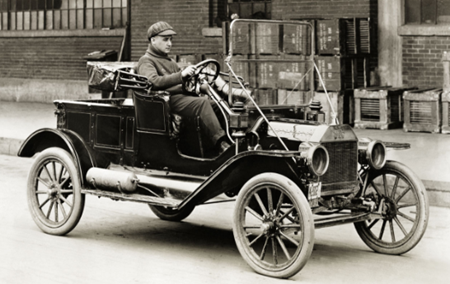
\includegraphics[width=5.62in]{./image/carroantigo} \end{center}

\url{http://unusual-cars.com/wp-content/uploads/2016/01/Ford-Model-T-1908.jpg}

ANOVA (sigla, do inglês, Analysis of Variance) utiliza a estatística
\(F\).

\begin{itemize}
\tightlist
\item
  A ANOVA de Fisher é uma extensão do teste \(t\), com:

  \begin{itemize}
  \tightlist
  \item
    VI (variável independente) nominal com \textbf{três ou mais}
    categorias (politômica nominal, fator)
  \item
    VD (variável dependente) quantitativa (unifatorial, \emph{One way}
    ANOVA)
  \end{itemize}
\item
  Pode ser:

  \begin{itemize}
  \tightlist
  \item
    independente (fator entre participantes)
  \item
    relacionada (fator intraparticipantes)
  \end{itemize}
\end{itemize}

O tamanho do efeito é expresso pelo eta ao quadrado (\(\eta^2\)).

\begin{center}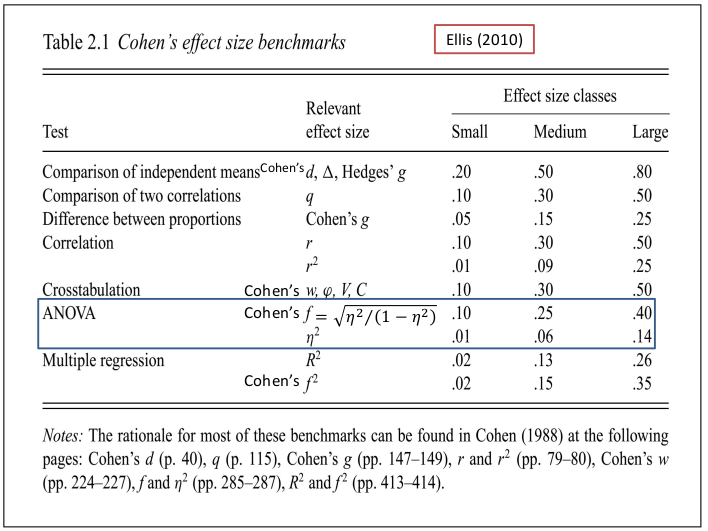
\includegraphics[width=4.72in]{./image/ANOVA_efeitos} \end{center}

\begin{center}\rule{0.5\linewidth}{\linethickness}\end{center}

\begin{flushleft}
\includegraphics[width=0.67in]{./image/coruja} \end{flushleft}

Tradicionalmente exigia-se, para a ANOVA clássica, que a distribuição
populacional da variável fosse normal para cada condição e que existisse
homocedasticidade entre os grupos. Estas premissas eram testadas:

\begin{itemize}
\tightlist
\item
  Normalidade da VD (teste de Shapiro-Wilk) se a amostra fosse pequena.
\item
  Homocedasticidade (teste de Levene) se os grupos fossem
  desbalanceados.
\end{itemize}

Quando as premissas não eram atendidas, recomendava-se o teste não
paramétrico H de Kruskal-Wallis.

\begin{center}\rule{0.5\linewidth}{\linethickness}\end{center}

ANOVA é relativamente robusta às violações das suposições de
normalidade, homocedasticidade e \emph{outliers}.

Se o tamanho da amostra é pequeno, ou há heterocedasticidade,
desbalanceamento, ou assimetria da VD, deve-se considerar a execução de
uma ANOVA de Welch, ou ANOVA não-paramétrica ou ANOVA com reamostragem
(\emph{bootstrapping}).

\subsection{- é necessário seguir as premissas com todo o
rigor?}\label{e-necessario-seguir-as-premissas-com-todo-o-rigor}

Ilustramos com uma analogia, recordando o equilíbrio de Hardy-Weinberg.

\begin{center}\rule{0.5\linewidth}{\linethickness}\end{center}

\textbf{The Hardy-Weinberg Law of Genetic Equilibrium}

In 1908 G. Hardy and W. Weinberg independently proposed that the
frequency of alleles and genotypes in a population will remain constant
from generation to generation if the population is stable and in genetic
equilibrium. Five conditions are required in order for a population to
remain at Hardy-Weinberg equilibrium:

\begin{itemize}
\tightlist
\item
  A large breeding population
\item
  Random mating
\item
  No change in allelic frequency due to mutation
\item
  No immigration or emigration
\item
  No natural selection
\end{itemize}

\url{http://www.phschool.com/science/biology_place/labbench/lab8/concepts.html}

\begin{center}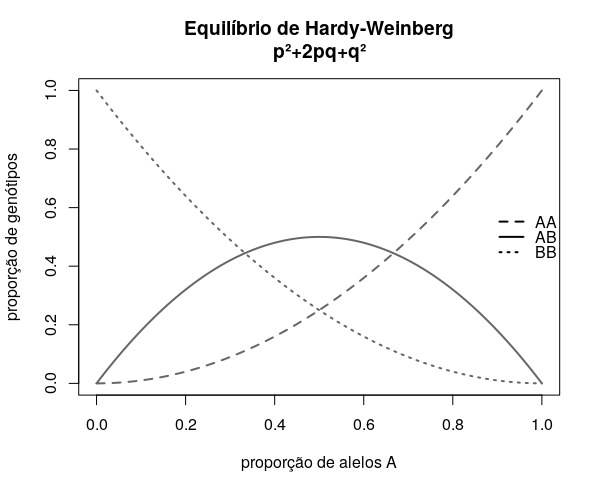
\includegraphics[width=5.45in]{./image/HW_teoria} \end{center}

\begin{center}\rule{0.5\linewidth}{\linethickness}\end{center}

Violando as condições de H-W, em simulação com:

\begin{itemize}
\tightlist
\item
  500 indivíduos,
\item
  mutação alterando a frequência dos alelos,
\item
  selecionando para o alelo \textbf{A}.
\end{itemize}

\begin{Shaded}
\begin{Highlighting}[]
\KeywordTok{source}\NormalTok{(}\StringTok{"HardyWeinberg.R"}\NormalTok{)}
\end{Highlighting}
\end{Shaded}

Observamos, por exemplo:

\begin{center}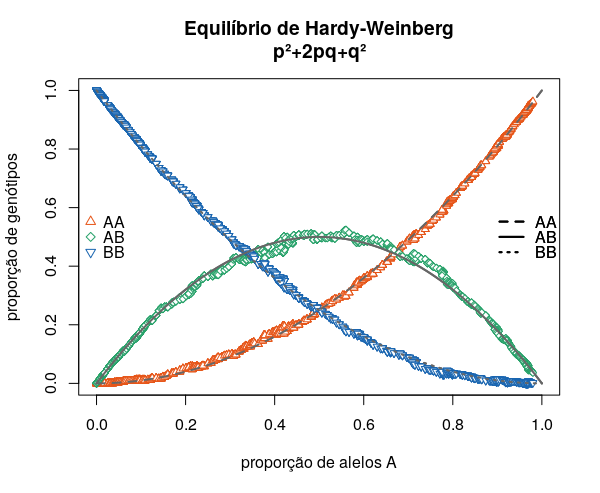
\includegraphics[width=5.45in]{./image/HW} \end{center}

As condições matemáticas de população muito grande (ou infinita), sem
mutação e sem seleção garantem a população no equilíbrio de
Hardy-Weinberg; porém, dentro de certos limites, ainda encontramos
predição aceitável para o Equilíbrio de Hardy-Weinberg e poderíamos
utilizá-los em populações biológicas.

\subsection{- o que é independência?}\label{o-que-e-independencia}

Um delineamento independente é aquele em que cada unidade experimental
só é submetida a uma condição experimental.

Por exemplo, três grupos com 5 indivíduos cada um (total de 15
participantes, nomeados de A a J) são alocados assim:

 Condição 1

 Condição 2

 Condição 3

A

F

K

B

G

L

C

H

M

D

I

N

E

J

O

Em um delineamento relacionado, o mesmo indivíduo é submetido a todas as
condições experimentais. Os mesmos 15 participantes seriam alocados
assim:

 Condição 1

 Condição 2

 Condição 3

A

A

A

B

B

B

C

C

C

D

D

D

E

E

E

F

F

F

G

G

G

H

H

H

I

I

I

J

J

J

K

K

K

L

L

L

M

M

M

N

N

N

O

O

O

\subsection{- o que é balanceamento?}\label{o-que-e-balanceamento}

Em delineamentos em que os grupos são balanceados, o número de
participantes em cada condição é aproximadamente igual. Por exemplo, com
15 participantes em ANOVA independente, desbalanceada, poderíamos ter
algo como.

 Condição 1

 Condição 2

 Condição 3

A

H

K

B

I

L

C

J

M

D

N

E

O

F

G

Em um delineamento intra-participantes o desbalanceamento ocorre quando
um dos participantes deixa de aparecer em uma das condições
experimentais, por exemplo:

 Condição 1

 Condição 2

 Condição 3

A

A

A

B

B

C

C

C

D

D

D

E

E

E

F

F

F

G

G

G

H

H

H

I

I

I

J

J

K

K

K

L

L

L

M

M

M

N

N

N

O

O

O

Basta uma participação faltando (\emph{missing}) para caracterizar o
desbalanceamento. O procedimento com as estatísticas padrão do R não
funcionarão e temos que usar um modelo com efeitos aleatórios; lidaremos
com esta situação adiante.

\section{\texorpdfstring{Distribuição \(F\) de
Fisher-Snedecor}{Distribuição F de Fisher-Snedecor}}\label{distribuicao-f-de-fisher-snedecor}

Esta distribuição é uma generalização da estatística \(t\) para três ou
mais grupos. Descreve probabilidades que dependem da razão entre duas
variâncias, e portanto considera graus de liberdade (\(\nu\), letra
grega \emph{\href{https://pt.wikipedia.org/wiki/\%CE\%9D}{ni}} ) para o
numerador e para o denominador.

Para a comparação de três ou mais condições, com base na estatística
\(F\), os graus de liberdade do numerador dependem do número de
condições e os do denominador dependem do tamanho da amostra.

Familiarize-se com a distribuição \(F\), observando
\emph{\url{Animacao_F.R}}:

\begin{itemize}
\tightlist
\item
  \(F\) é um valor maior que zero.
\item
  sob \(H_0\) a distribuição \(F\) tem um parâmetro de não centralidade
  (ncp) igual a zero; sob \(H_1\) o parâmetro de não centralidade é
  maior do que zero.
\item
  esta distribuição é assimétrica.
\item
  consideramos somente a cauda superior.
\item
  localize \(\alpha\) e \(\beta\).
\item
  há dois valores para graus de liberdade: para o numerador (número de
  grupos - 1) e denominador (número de sujeitos - número de grupos).
\item
  observe o que acontece com a distribuição sob \(H_0\) e com o valor de
  \(F\) crítico (\(F_c\)) à medida que os graus de liberdade aumentam.
\end{itemize}

O delineamento dos estudos, o tipo de variável e, consequentemente, a
estatística adequada mudam, mas o problema é sempre o mesmo: incerteza
porque lidamos com uma amostra.

\begin{center}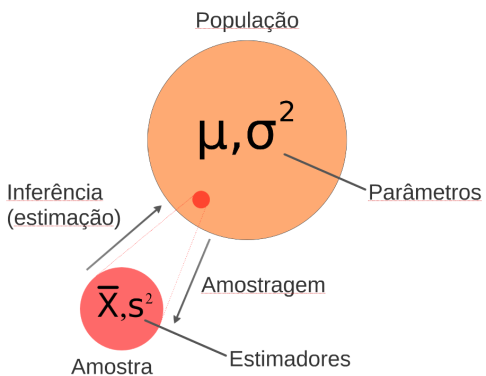
\includegraphics[width=2.86in]{./image/pop_amostra} \end{center}

A diferença, aqui, é que teremos que lidar com 3 ou mais amostras
simultaneamente.

\begin{center}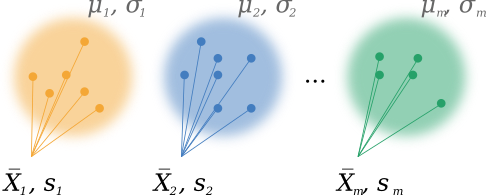
\includegraphics[width=4.42in]{./image/pop_amostra_3} \end{center}

A hipótese nula é pela igualdade de todos os \(m\) grupos. caso não
rejeitemos \(H_0\):

\begin{center}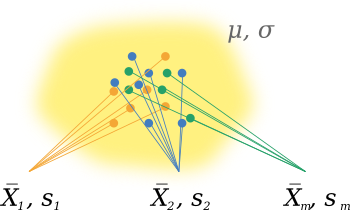
\includegraphics[width=3.18in]{./image/pop_amostra_3_H0} \end{center}

Quando rejeitamos \(H_0\) assumimos que todas as condições são
diferentes entre si:

\begin{center}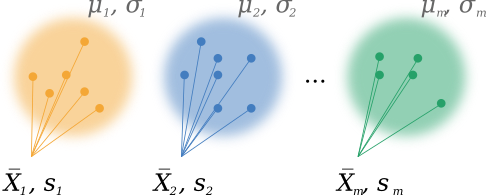
\includegraphics[width=4.42in]{./image/pop_amostra_3} \end{center}

ou

que pelo menos uma destoe das demais (i.e., basta que uma das condições
ser diferente das demais para rejeitarmos \(H_0\).), por exemplo:

\begin{center}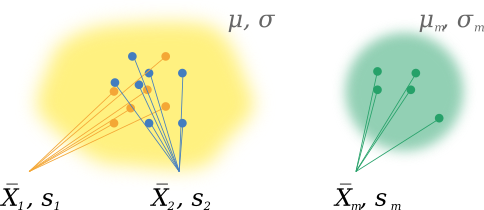
\includegraphics[width=4.4in]{./image/pop_amostra_3_H1} \end{center}

\subsection{\texorpdfstring{teste \(t\) (quando eram duas
turmas)}{teste t (quando eram duas turmas)}}\label{teste-t-quando-eram-duas-turmas}

Brendon Small e Coach McGuirk fazem com que seus alunos do SNAP-Ed
mantenham diários do que comem por uma semana e depois calculem a
ingestão diária de sódio em miligramas.

Desde que as classes receberam diferentes programas de educação
nutricional, eles querem ver se a ingestão média de sódio é a mesma para
as duas turmas.

Aplicamos o teste \(t\) de Satterthwaite (\emph{a.k.a.} Welch), robusto
e \emph{default} do R:

\begin{Shaded}
\begin{Highlighting}[]
\CommentTok{# dados}
\KeywordTok{library}\NormalTok{(readxl)}
\NormalTok{Dtfrm <-}\StringTok{ }\KeywordTok{read_excel}\NormalTok{(}\StringTok{"Nutricao.xlsx"}\NormalTok{)}
\CommentTok{# significancia estatistica}
\NormalTok{t_out <-}\StringTok{ }\KeywordTok{t.test}\NormalTok{(Sodium }\OperatorTok{~}\StringTok{ }\NormalTok{Instructor, }\DataTypeTok{data =}\NormalTok{ Dtfrm)}
\KeywordTok{print}\NormalTok{(t_out)}
\end{Highlighting}
\end{Shaded}

\begin{verbatim}

    Welch Two Sample t-test

data:  Sodium by Instructor
t = 0.76722, df = 34.893, p-value = 0.4481
alternative hypothesis: true difference in means is not equal to 0
95 percent confidence interval:
 -67.91132 150.41132
sample estimates:
mean in group Brendon Small mean in group Coach McGuirk 
                    1287.50                     1246.25 
\end{verbatim}

\subsubsection{\texorpdfstring{testes \(t\) quando temos três ou mais
turmas}{testes t quando temos três ou mais turmas}}\label{testes-t-quando-temos-tres-ou-mais-turmas}

Suponha que uma terceira classe junte-se ao experimento (Melissa
Robins). Podemos, então, verificar as diferenças destas três condições
experimentais com testes \(t\), comparando-se Brendon Small com Coach
McGuirk, Brendon Small com Melissa Robins e Coach McGuirk com Melissa
Robins?

 Quantos testes \(t\) precisaremos de acordo com o número de grupos?

\begin{center}
\includegraphics[width=1.84in]{./image/hammer} \end{center}

\url{https://www.toolsbr.com.br/produto/dewalt-martelo-20-oz-rip-claw-hammer-94480}

É a combinatória do número de grupos (\(m\)) dois a dois:
\[{m \choose 2} = { {m!} \over {2! (m-2)!} }\]

\begin{itemize}
\tightlist
\item
  para 2 -grupos:
  \({2 \choose 2} = { {2!} \over {2! (2-2)!} } = 1~\text{teste}\)
\end{itemize}

\begin{center}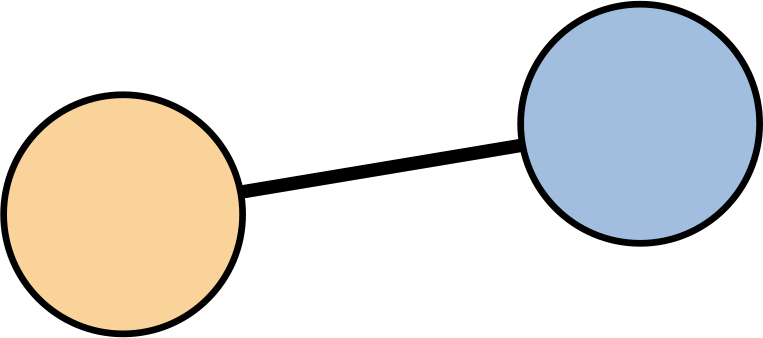
\includegraphics[width=0.76in]{./image/t2} \end{center}

\begin{itemize}
\tightlist
\item
  para 3 grupos:
  \({3 \choose 2} = { {3!} \over {2! (3-2)!} } = 3~\text{testes}\)
\end{itemize}

\begin{center}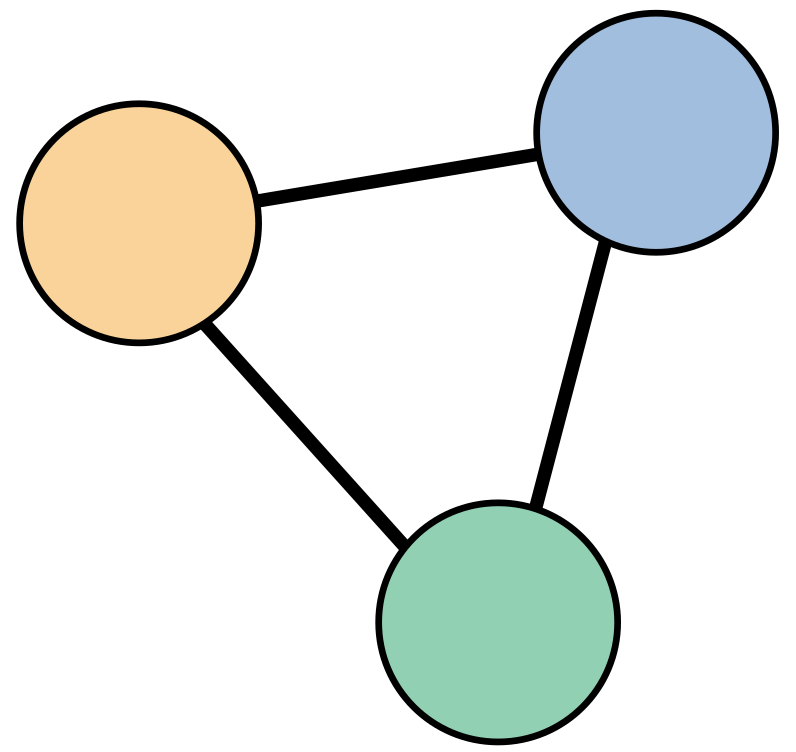
\includegraphics[width=0.8in]{./image/t3} \end{center}

\begin{itemize}
\tightlist
\item
  para 4 grupos:
  \({4 \choose 2} = { {4!} \over {2! (4-2)!} } = 6~\text{testes}\)
\end{itemize}

\begin{center}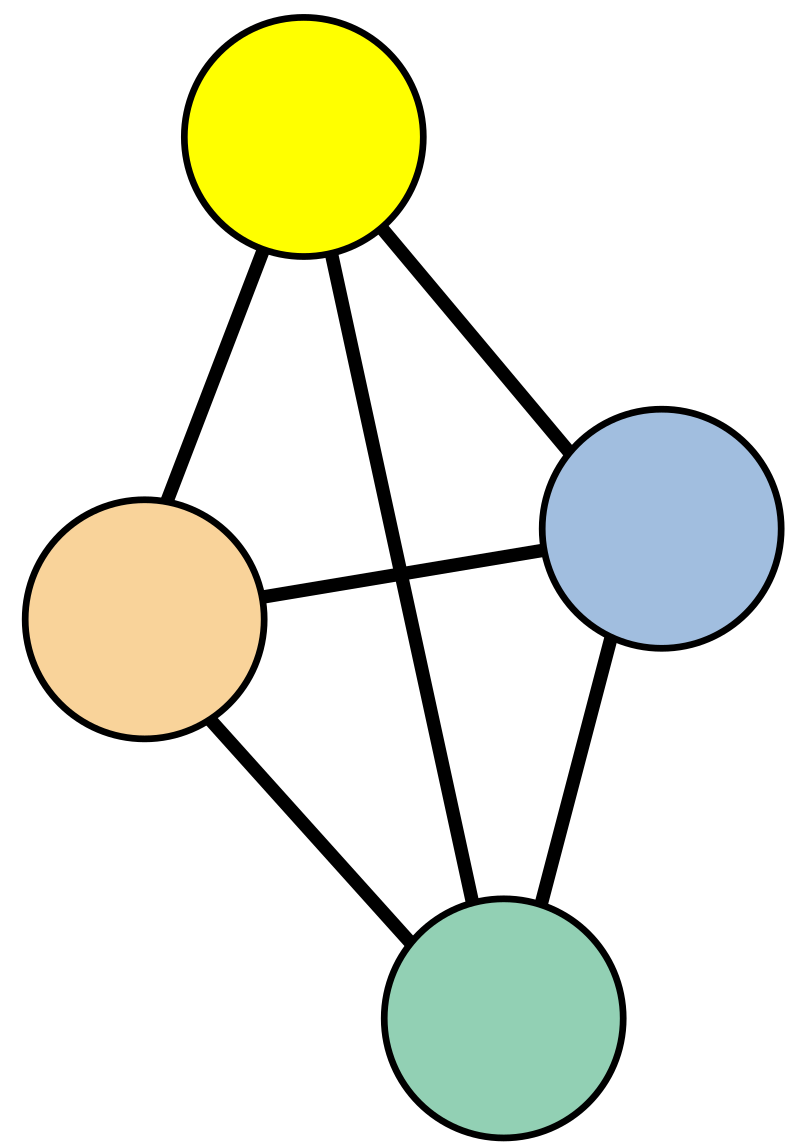
\includegraphics[width=0.81in]{./image/t4} \end{center}

\begin{itemize}
\tightlist
\item
  para 6 grupos:
  \({6 \choose 2} = { {6!} \over {2! (6-2)!} } = 15~\text{testes}\)
\end{itemize}

\begin{center}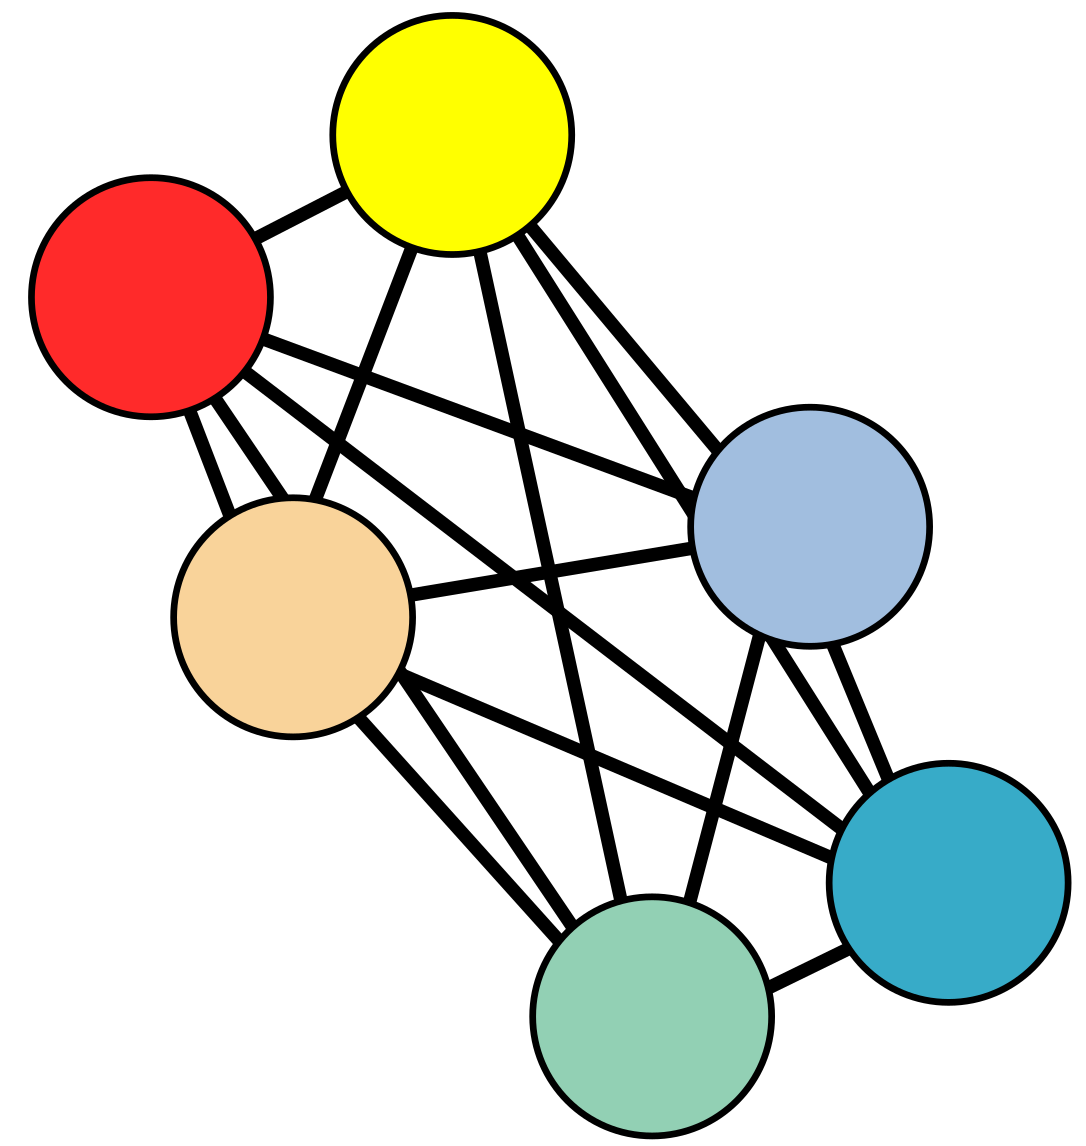
\includegraphics[width=1.09in]{./image/t6} \end{center}

Graficamente vemos:

\begin{Shaded}
\begin{Highlighting}[]
\CommentTok{# Testes_t_2a2.R}
\CommentTok{# Ilustra o numero de testes t necessarios}
\CommentTok{# para comparar grupos par a par}

\NormalTok{combinacoes <-}\StringTok{ }\KeywordTok{c}\NormalTok{()}
\NormalTok{grupos <-}\StringTok{ }\KeywordTok{c}\NormalTok{()}
\ControlFlowTok{for}\NormalTok{ (g }\ControlFlowTok{in} \DecValTok{2}\OperatorTok{:}\DecValTok{20}\NormalTok{)}
\NormalTok{\{}
\NormalTok{  grupos <-}\StringTok{ }\KeywordTok{c}\NormalTok{(grupos,g)}
\NormalTok{  combinacoes <-}\StringTok{ }\KeywordTok{c}\NormalTok{(combinacoes,}\KeywordTok{choose}\NormalTok{(g,}\DecValTok{2}\NormalTok{))}
\NormalTok{\}}
\KeywordTok{plot}\NormalTok{(grupos,combinacoes,}
     \DataTypeTok{xlab=}\StringTok{"Número de grupos"}\NormalTok{,}
     \DataTypeTok{ylab=}\StringTok{"Número de testes t feitos par a par"}\NormalTok{,}
     \DataTypeTok{lwd=}\DecValTok{2}\NormalTok{,}
     \DataTypeTok{type=}\StringTok{"b"}\NormalTok{)}
\end{Highlighting}
\end{Shaded}

\begin{center}\includegraphics{TresMaisCondicoes_files/figure-latex/unnamed-chunk-18-1} \end{center}

Embora o número cresça rapidamente, podemos não nos impressionar pois
temos computadores para o trabalho repetitivo. Há, porém, um problema
mais grave: as probabilidades dos erros do tipo I (\(\alpha\)) e do tipo
II (\(\beta\)) se acumulam. Quando escolhemos \(\alpha\), \textbf{a
probabilidade de rejeitar incorretamente a hipótese nula}, o máximo
valor que \(p\) pode assumir, a probabilidade deste erro para \(m\)
grupos é:

\[P(\alpha | m) = 1-(1-\alpha)^{m \choose 2}\]

Também gostaríamos de manter a \textbf{probabilidade de rejeitar
corretamente a hipótese nula}, o poder do teste, \(1-\beta\); para \(m\)
grupos é:

\[P(\beta | m) = (1-\beta) ^ {m \choose 2}\]

Graficamente podemos observar o que acontece com o número crescente de
pares de teste \(t\) necessários, considerando os tradicionais
\(\alpha=0.05\) e \(\beta=0.1\):

\begin{Shaded}
\begin{Highlighting}[]
\CommentTok{# Testes_t_AlfaPoder.R}
\CommentTok{# Ilustra o valor de alfa e 1-beta}
\CommentTok{# com numero crescente de testes }

\KeywordTok{source}\NormalTok{(}\StringTok{"friendlycolor.R"}\NormalTok{)}

\NormalTok{cor_alfa <-}\StringTok{ }\KeywordTok{friendlycolor}\NormalTok{(}\DecValTok{8}\NormalTok{)}
\NormalTok{cor_poder <-}\StringTok{ }\KeywordTok{friendlycolor}\NormalTok{(}\DecValTok{20}\NormalTok{)}

\NormalTok{alfa_escolhido <-}\StringTok{ }\FloatTok{0.05}
\NormalTok{beta_escolhido <-}\StringTok{ }\FloatTok{0.20}
\NormalTok{alfa <-}\StringTok{ }\KeywordTok{c}\NormalTok{()}
\NormalTok{poder <-}\StringTok{ }\KeywordTok{c}\NormalTok{()}
\NormalTok{grupos <-}\StringTok{ }\KeywordTok{c}\NormalTok{()}
\ControlFlowTok{for}\NormalTok{ (g }\ControlFlowTok{in} \DecValTok{2}\OperatorTok{:}\DecValTok{20}\NormalTok{)}
\NormalTok{\{}
\NormalTok{  grupos <-}\StringTok{ }\KeywordTok{c}\NormalTok{(grupos,g)}
\NormalTok{  combinacoes <-}\StringTok{ }\KeywordTok{choose}\NormalTok{(g,}\DecValTok{2}\NormalTok{)}
  
\NormalTok{  alfa <-}\StringTok{ }\KeywordTok{c}\NormalTok{(alfa,}\DecValTok{1}\OperatorTok{-}\NormalTok{(}\DecValTok{1}\OperatorTok{-}\NormalTok{alfa_escolhido)}\OperatorTok{^}\NormalTok{combinacoes)}
\NormalTok{  poder <-}\StringTok{ }\KeywordTok{c}\NormalTok{(poder,(}\DecValTok{1}\OperatorTok{-}\NormalTok{beta_escolhido)}\OperatorTok{^}\NormalTok{combinacoes)}
\NormalTok{\}}
\KeywordTok{plot}\NormalTok{(grupos, poder,}
     \DataTypeTok{xlab=}\StringTok{"Número de grupos"}\NormalTok{,}
     \DataTypeTok{ylab=}\StringTok{"Probabilidade"}\NormalTok{,}
     \DataTypeTok{ylim=}\KeywordTok{c}\NormalTok{(}\DecValTok{0}\NormalTok{,}\DecValTok{1}\NormalTok{),}
     \DataTypeTok{lwd=}\DecValTok{2}\NormalTok{, }\DataTypeTok{lty=}\DecValTok{2}\NormalTok{, }\DataTypeTok{col=}\NormalTok{cor_poder,}
     \DataTypeTok{type=}\StringTok{"b"}\NormalTok{)}
\KeywordTok{lines}\NormalTok{(grupos,alfa,}
      \DataTypeTok{lwd=}\DecValTok{2}\NormalTok{, }\DataTypeTok{lty=}\DecValTok{1}\NormalTok{, }\DataTypeTok{col=}\NormalTok{cor_alfa, }
      \DataTypeTok{type=}\StringTok{"b"}\NormalTok{)}
\KeywordTok{legend}\NormalTok{(}\StringTok{"right"}\NormalTok{,}
       \KeywordTok{c}\NormalTok{(}\StringTok{"alfa"}\NormalTok{, }\StringTok{"poder"}\NormalTok{),}
       \DataTypeTok{col=}\KeywordTok{c}\NormalTok{(cor_alfa,cor_poder),}
       \DataTypeTok{lwd=}\KeywordTok{c}\NormalTok{(}\DecValTok{2}\NormalTok{,}\DecValTok{2}\NormalTok{),}
       \DataTypeTok{lty=}\KeywordTok{c}\NormalTok{(}\DecValTok{1}\NormalTok{,}\DecValTok{2}\NormalTok{),}
       \DataTypeTok{box.lwd=}\DecValTok{0}\NormalTok{, }\DataTypeTok{bg=}\StringTok{"transparent"}\NormalTok{)}
\end{Highlighting}
\end{Shaded}

\begin{center}\includegraphics{TresMaisCondicoes_files/figure-latex/unnamed-chunk-19-1} \end{center}

Portanto, a probabilidade de erro do tipo I cresce rapidamente para
quase \(100\%\) e o poder de seus testes combinados vai para zero. Na
prática, dificilmente teremos mais do que 6 grupos mas, ainda assim,
teríamos \(\alpha \approx 53.7\%\) e poder \(1-\beta \approx 3.5\%\),
valores totalmente inaceitáveis para uma boa análise.

 Podemos resolver com vários testes \(t\)? A resposta é:

\begin{center}
\includegraphics[width=2.56in]{./image/meme_NO} \end{center}

NÃO!

Precisamos testar tudo simultaneamente para manter \(\alpha\) no valor
pretendido e preservar \(1-\beta\).

\section{Análise da variância}\label{analise-da-variancia}

Esta análise, que tem o acrônimo ANOVA (do inglês, \textbf{An}alysis
\textbf{o}f \textbf{Va}riance) utiliza apenas variâncias, mas\ldots{}

 \ldots{} as conclusões são sobre as médias dos \(m\) grupos.

Como?

\begin{center}
\includegraphics[width=2.26in]{./image/bebesurpreso} \end{center}

\subsection{Princípio do teste ANOVA
unifatorial}\label{principio-do-teste-anova-unifatorial}

Consideremos que existam três grupos com distribuição normal. De cada um
deles, retiramos uma amostra:

\begin{center}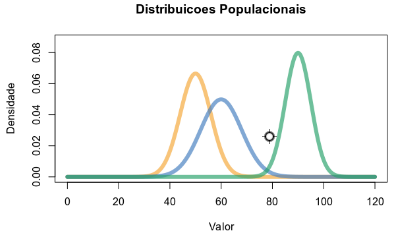
\includegraphics[width=3.64in]{./image/pop3} \end{center}

\begin{center}
\includegraphics[width=3.64in]{./image/amo3} \end{center}

Não havendo problemas, as três amostras reproduzem a distribuição, média
e variância das populações das quais se originaram.

A distribuição \(F\) é dada por \[F = {{S_E^2}\over{S_D^2}}\] onde
\(S_E^2\) é a variância \textbf{entre} os grupos e \(S_D^2\) é a
variância \textbf{dentro} dos grupos.

\subsubsection{\texorpdfstring{Variância entre (\emph{between}) os
grupos}{Variância entre (between) os grupos}}\label{variancia-entre-between-os-grupos}

A variância entre os grupos presume que as médias amostrais
(\(\bar{X}_m\)) refletem as respectivas médias populacionais
(\(\mu_m\)):

\begin{center}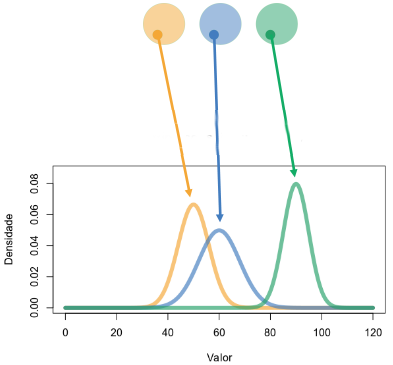
\includegraphics[width=3.57in]{./image/variancia_entre} \end{center}

Como sempre, não temos esta certeza e lidamos somente com a informação
das amostras, \(\bar{X}_m\):

\begin{center}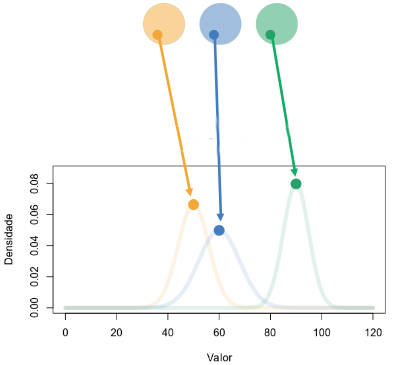
\includegraphics[width=3.57in]{./image/variancia_entre_amo} \end{center}

Cada média é um número e, portanto, podemos calcular a variância destes
números:

\begin{center}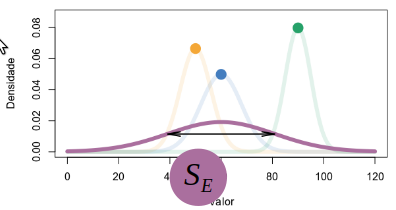
\includegraphics[width=3.6in]{./image/variancia_entre_SE} \end{center}

\begin{center}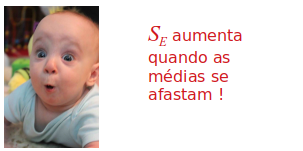
\includegraphics[width=2.75in]{./image/bebesurpreso_SE} \end{center}

Sendo assim, para \(F = {{S_E^2}\over{S_D^2}}\), a estatística \(F\)
aumenta quando a variância entre os grupos (ou condições) aumentar.

\subsubsection{\texorpdfstring{Variância dentro (\emph{within}) dos
grupos}{Variância dentro (within) dos grupos}}\label{variancia-dentro-within-dos-grupos}

A variância dentro dos grupos é uma medida da variância total,
desconsiderando a média de cada uma das condições. Cada amostra tem sua
própria distribuição (presumivelmente, reflexo da distribuição da
população de onde veio):

\begin{center}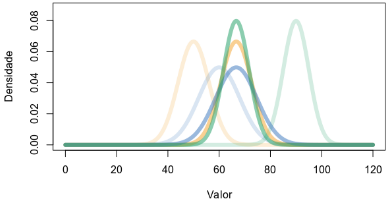
\includegraphics[width=3.55in]{./image/variancia_dentro} \end{center}

Como sempre, não temos esta certeza e lidaremos somente com a informação
das amostras, \(\S_m\):

\begin{center}
\includegraphics[width=3.55in]{./image/variancia_dentro_amo} \end{center}

Mesclando as três distribuições, estimamos a variância dentro dos
grupos, \(S_D^2\), uma medida de quanto, como um todo, a variável é
dispersa:

\begin{center}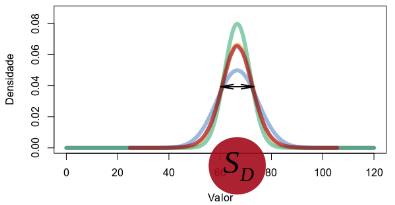
\includegraphics[width=3.59in]{./image/variancia_dentro_SD} \end{center}

Caso a variância em cada condição seja maior,

\begin{center}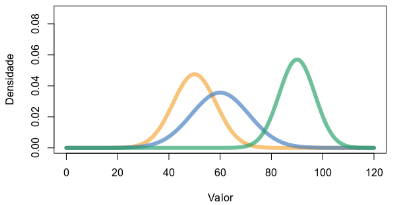
\includegraphics[width=3.59in]{./image/variancia_dentro_SD3} \end{center}

esta variância será refletida em \(S_D^2\):

\begin{center}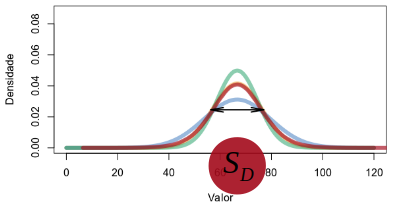
\includegraphics[width=3.59in]{./image/variancia_dentro_SDmais} \end{center}

\begin{center}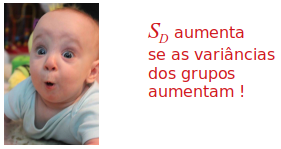
\includegraphics[width=2.55in]{./image/bebesurpreso_SD} \end{center}

Sendo assim, para \(F = {{S_E^2}\over{S_D^2}}\), a estatística \(F\)
diminui quando a variância dentro os grupos (ou condições) aumentar.

\subsection{\texorpdfstring{Comportamento de
\(F = {{S_E^2}\over{S_D^2}}\)}{Comportamento de F = \{\{S\_E\^{}2\}\textbackslash{}over\{S\_D\^{}2\}\}}}\label{comportamento-de-f-s_e2overs_d2}

É fácil imaginar o comportamento da estatística \(F\) combinando-se o
que pode acontecer com \(S_E^2\) e \(S_D^2\):

\begin{center}\rule{0.5\linewidth}{\linethickness}\end{center}

\begin{center}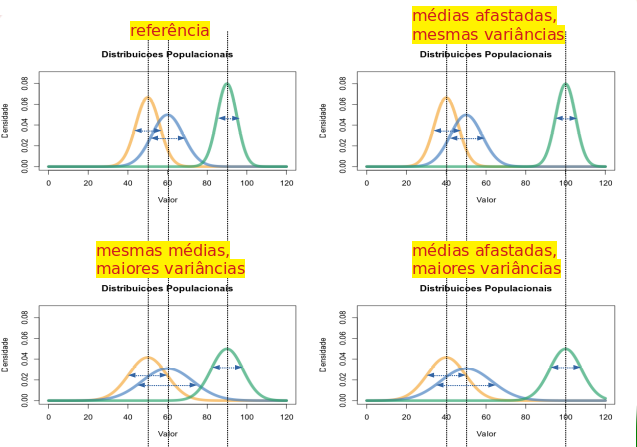
\includegraphics[width=5.79in]{./image/F_X_s} \end{center}

\begin{center}\rule{0.5\linewidth}{\linethickness}\end{center}

\begin{center}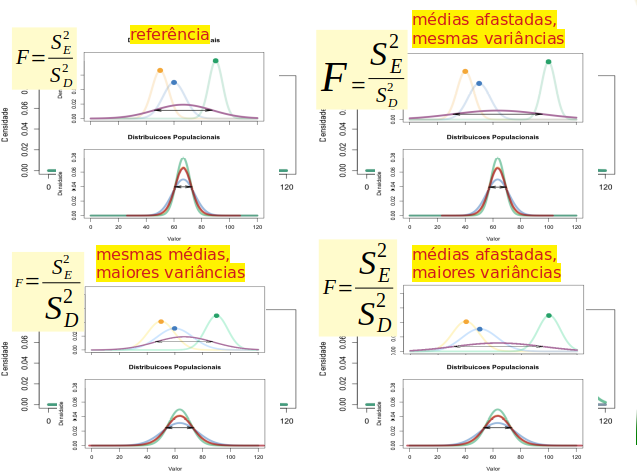
\includegraphics[width=5.79in]{./image/F_SE_SD} \end{center}

\begin{center}\rule{0.5\linewidth}{\linethickness}\end{center}

Desta forma, Ronald Fisher inventou uma forma de comparar médias entre
várias condições, simultaneamente, utilizando somente a comparação entre
duas variâncias, com o numerador refletindo a dispersão das médias e o
denominador refletindo a dispersão do fenômeno em estudo.

\begin{center}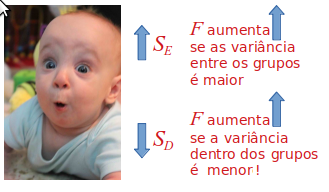
\includegraphics[width=2.99in]{./image/bebesurpreso_F} \end{center}

\section{Métodos Robustos}\label{metodos-robustos}

\begin{center}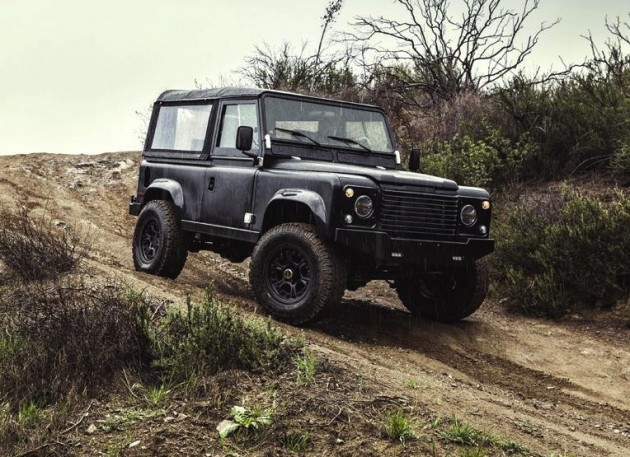
\includegraphics[width=7.88in]{./image/defender} \end{center}

\url{https://performancedrive.com.au/icon-land-rover-defender-90-6-2-chev-v8-1606/}

\section{ANOVA para condições
independentes}\label{anova-para-condicoes-independentes}

Utilizada quando os participantes são avaliados em somente uma das
condições experimentais, i.e., um delineamento independente ou entre
participantes.

\subsection{- suposições}\label{suposicoes}

\begin{itemize}
\tightlist
\item
  independência entre as unidades experimentais,
\item
  normalidade da VD em todas as condições,
\item
  homocedasticidade da VD entre todas as condições.
\end{itemize}

\begin{center}\rule{0.5\linewidth}{\linethickness}\end{center}

\begin{flushleft}
\includegraphics[width=0.67in]{./image/coruja} \end{flushleft}

\textbf{Normalidade e balanceamento}:

\begin{quote}
``O teste t é ainda um teste válido, mesmo com modestas violações na
suposição de normalidade, particularmente quando os tamanhos dos grupos
são iguais e existe um número razoável de participantes em cada grupo;
por ``razoável'' entendemos que, em um delineamento completamente entre
participantes, deve haver pelo menos 12 participantes por
grupo{[}\ldots{}{]}'' (Dancey \& Reidy, 2019, p.~472)
\end{quote}

Então: - se o número de unidades experimentais é igual a pelo menos 12
em cada grupo, a suposição de normalidade não é necessária.

\begin{itemize}
\tightlist
\item
  se os grupos são balanceados, homocedasticidade não é necessária.
\end{itemize}

\begin{center}\rule{0.5\linewidth}{\linethickness}\end{center}

O balanceamento não precisa ser estrito:

\begin{quote}
``Consideram-se grupos de dimensão semelhante quando o quociente entre a
maior dimensão e a menor for inferior a 1,5.'' (Pestana, M. \& Gageiro,
J. (2008) Análise de dados para Ciências Sociais: a complementaridade do
SPSS. Lisboa: Sílabo, p.~278)
\end{quote}

Então:

\begin{itemize}
\tightlist
\item
  Se a maior quantidade de unidades observacionais numa condição NÃO
  superar 1,5 vezes a condição de menor quantidade de unidades
  observacionais, então a suposição de homocedasticidade não precisa ser
  considerada para o teste ANOVA unifatorial independente.
\end{itemize}

\begin{center}\rule{0.5\linewidth}{\linethickness}\end{center}

\begin{center}\rule{0.5\linewidth}{\linethickness}\end{center}

\begin{flushleft}
\includegraphics[width=0.67in]{./image/coruja} \end{flushleft}

\textbf{Homocedasticidade}:

Em geral, quando você tiver tamanhos de amostras iguais, a suposição de
homocedasticidade não será um grande problema.

- Dancey \& Reidy (2019), p.~472-3

\begin{itemize}
\tightlist
\item
  ANOVA unifatorial independente de Fisher para condições
  \textbf{balanceadas} é adequada na situação de heterocedasticidade
  populacional.
\item
  ANOVA unifatorial independente de Welch para condições
  \textbf{desbalanceadas} é adequada na situação de heterocedasticidade
  populacional.
\end{itemize}

A homocedasticidade ocorre heuristicamente se (maior
desvio-padrão)/(menor desvio-padrão) é maior que 2.

- Johnson, R. \& Wichern, D. (2007) Applied Multivariate Statistical
Analysis. 6 th ed. NJ: Prentice-Hall, p.~291

- Moore, D. (1995) The basic practice of statistics. New York: W. H.
Freeman and Company, citado por Norusis, M. (2009) PASW Statistics 18:
Statistics Procedures Companion. NJ: Prentice-Hall, p.~148

\begin{center}\rule{0.5\linewidth}{\linethickness}\end{center}

\subsection{- situação}\label{situacao}

\begin{flushleft}
\includegraphics[width=1.07in]{./image/snaped} \end{flushleft}

\url{https://www.fns.usda.gov/snap/supplemental-nutrition-assistance-program-education-snap-ed}

O SNAP-Ed (Supplemental Nutrition Assistance Program Education) é um
programa baseado em evidências que ajuda as pessoas a terem uma vida
mais saudável.

O SNAP-Ed ensina às pessoas que usam ou qualificam para o SNAP uma boa
nutrição e como fazer com que o seu dinheiro de alimentação se estenda
ainda mais.

Os participantes do SNAP-Ed também aprendem a ser fisicamente ativos.

\subsection{- planejamento}\label{planejamento}

Brendon Small, Coach McGuirk e Melissa Robins fazem com que seus alunos
do SNAP-Ed mantenham diários do que comem por uma semana e depois
calculem a ingestão diária de sódio em miligramas.

Desde que as classes receberam diferentes programas de educação
nutricional, eles querem ver se a ingestão média de sódio é a mesma para
as três turmas.

\subsection{- hipóteses nula e
alternativa}\label{hipoteses-nula-e-alternativa}

As três classes receberam diferentes programas de educação nutricional.
A ingestão média de sódio é a mesma (populacionalmente) para os três
programas?

\[H_0: \mu_{\text{Small}} = \mu_{\text{McGuirk}} = \mu_{\text{Robins}}\]
\[H_1: \exists |\mu_i \ne \mu_j; i \ne j; i,j=1,2,3\]

\begin{center}\rule{0.5\linewidth}{\linethickness}\end{center}

\begin{flushleft}
\includegraphics[width=0.67in]{./image/coruja} \end{flushleft}

Esta é uma forma matemática para escrever a hipótese alternativa, lida
como ``Existe pelo menos alguma média \(\mu_i\), diferente de outra
média \(\mu_j\), com \(i\) e \(j\) assumindo os valores \(1\), \(2\) ou
\(3\)''. É dizer que \(\mu_1 \ne \mu_2\) \textbf{OU} \(\mu_1 \ne \mu_3\)
\textbf{OU} \(\mu_2 \ne \mu_3\).

Aparece, por aí, como: \[H_1: \mu_1 \ne \mu_2 \ne \mu_3\] tentando
indicar as diferenças, mas esta forma não funciona porque sugere que a
rejeição de \(H_0\) implica em que todos os grupos sejam diferentes
entre si, como \(\mu_1 \ne \mu_2\) \textbf{E} \(\mu_1 \ne \mu_3\)
\textbf{E} \(\mu_2 \ne \mu_3\).

Basta que uma condição tenha média estatisticamente diferente das demais
para que se rejeite \(H_0\) com ANOVA. Em português:

\[H_1: \text{Existe pelo menos um grupo diferente de algum outro.}\]

\begin{center}\rule{0.5\linewidth}{\linethickness}\end{center}

\subsection{Operacionalização do
teste}\label{operacionalizacao-do-teste}

\subsubsection{ANOVA unifatorial independente de Fisher com ajuste para
heterocedasticidade de
White}\label{anova-unifatorial-independente-de-fisher-com-ajuste-para-heterocedasticidade-de-white}

A estatística descritiva e inferencial pode ser obtida com
\url{ANOVA1f_indep_FisherWhite_sodio.R}:

\begin{Shaded}
\begin{Highlighting}[]
\CommentTok{# ANOVA1f_indep_FisherWhite_sodio.R}
\CommentTok{# para ajustar este RScript para outros dados}
\CommentTok{# troque a planilha xlsx e substitua as palavras}
\CommentTok{# Instructor pela nova VI (fator)}
\CommentTok{# Sodium pela nova VD (resposta)}

\KeywordTok{library}\NormalTok{(psych)}
\KeywordTok{library}\NormalTok{(lattice)}
\KeywordTok{library}\NormalTok{(car)}
\KeywordTok{library}\NormalTok{(multcomp)}
\KeywordTok{library}\NormalTok{(gplots)}
\KeywordTok{library}\NormalTok{(emmeans)}
\KeywordTok{library}\NormalTok{(readxl)}

\CommentTok{# suppress warnings}
\KeywordTok{options}\NormalTok{(}\DataTypeTok{warn=}\OperatorTok{-}\DecValTok{1}\NormalTok{)}

\NormalTok{TH <-}\StringTok{ }\KeywordTok{read_excel}\NormalTok{(}\StringTok{"Nutricao3.xlsx"}\NormalTok{)}
\NormalTok{TH}\OperatorTok{$}\NormalTok{Instructor <-}\StringTok{ }\KeywordTok{factor}\NormalTok{(TH}\OperatorTok{$}\NormalTok{Instructor, }\DataTypeTok{levels=}\KeywordTok{unique}\NormalTok{(TH}\OperatorTok{$}\NormalTok{Instructor))}

\KeywordTok{print}\NormalTok{(}\KeywordTok{with}\NormalTok{(TH, psych}\OperatorTok{::}\KeywordTok{describeBy}\NormalTok{(Sodium,Instructor,}\DataTypeTok{digits=}\DecValTok{2}\NormalTok{)))}
\KeywordTok{boxplot}\NormalTok{(Sodium}\OperatorTok{~}\NormalTok{Instructor,}\DataTypeTok{data=}\NormalTok{TH,}
        \DataTypeTok{ylab=}\KeywordTok{names}\NormalTok{(TH)[}\KeywordTok{which}\NormalTok{(}\KeywordTok{names}\NormalTok{(TH)}\OperatorTok{==}\StringTok{"Sodium"}\NormalTok{)],}
        \DataTypeTok{xlab=}\KeywordTok{names}\NormalTok{(TH)[}\KeywordTok{which}\NormalTok{(}\KeywordTok{names}\NormalTok{(TH)}\OperatorTok{==}\StringTok{"Instructor"}\NormalTok{)]}
\NormalTok{)}
\KeywordTok{print}\NormalTok{(grf <-}\StringTok{ }\NormalTok{lattice}\OperatorTok{::}\KeywordTok{xyplot}\NormalTok{(Sodium}\OperatorTok{~}\NormalTok{Instructor, }\DataTypeTok{data=}\NormalTok{TH, }\DataTypeTok{type=}\KeywordTok{c}\NormalTok{(}\StringTok{"p"}\NormalTok{,}\StringTok{"a"}\NormalTok{),}
                             \DataTypeTok{jitter.x=}\OtherTok{TRUE}\NormalTok{, }\DataTypeTok{col=}\StringTok{"black"}\NormalTok{))}
\KeywordTok{with}\NormalTok{(TH, gplots}\OperatorTok{::}\KeywordTok{plotmeans}\NormalTok{(Sodium}\OperatorTok{~}\NormalTok{Instructor,}
                           \DataTypeTok{error.bars=}\StringTok{"conf.int"}\NormalTok{, }\DataTypeTok{level=}\NormalTok{.}\DecValTok{95}\NormalTok{,}
                           \DataTypeTok{connect=}\OtherTok{FALSE}\NormalTok{,}
                           \DataTypeTok{ylab=}\KeywordTok{names}\NormalTok{(TH)[}\KeywordTok{which}\NormalTok{(}\KeywordTok{names}\NormalTok{(TH)}\OperatorTok{==}\StringTok{"Sodium"}\NormalTok{)],}
                           \DataTypeTok{xlab=}\KeywordTok{names}\NormalTok{(TH)[}\KeywordTok{which}\NormalTok{(}\KeywordTok{names}\NormalTok{(TH)}\OperatorTok{==}\StringTok{"Instructor"}\NormalTok{)],}
                           \DataTypeTok{main=}\StringTok{"IC95%"}\NormalTok{,}
                           \DataTypeTok{barcol=}\StringTok{"black"}\NormalTok{))}
\NormalTok{car}\OperatorTok{::}\KeywordTok{densityPlot}\NormalTok{(Sodium}\OperatorTok{~}\NormalTok{Instructor, }\DataTypeTok{data=}\NormalTok{TH, }\DataTypeTok{rug=}\OtherTok{TRUE}\NormalTok{, }\DataTypeTok{from=}\DecValTok{0}\NormalTok{, }\DataTypeTok{normalize=}\OtherTok{TRUE}\NormalTok{,}
                 \DataTypeTok{na.rm=}\OtherTok{TRUE}\NormalTok{, }\DataTypeTok{ylab=}\StringTok{"Densidade"}\NormalTok{, }\DataTypeTok{col=}\KeywordTok{c}\NormalTok{(}\StringTok{"black"}\NormalTok{, }\StringTok{"black"}\NormalTok{, }\StringTok{"black"}\NormalTok{))}
\KeywordTok{cat}\NormalTok{(}\StringTok{"}\CharTok{\textbackslash{}n}\StringTok{"}\NormalTok{)}

\KeywordTok{cat}\NormalTok{(}\StringTok{"}\CharTok{\textbackslash{}n}\StringTok{ANOVA unifatorial independente de Fisher"}\NormalTok{,}
    \StringTok{"}\CharTok{\textbackslash{}n}\StringTok{com ajuste para heterocedasticidade de White:}\CharTok{\textbackslash{}n\textbackslash{}n}\StringTok{"}\NormalTok{)}
\NormalTok{alfa <-}\StringTok{ }\FloatTok{0.05}
\NormalTok{VD <-}\StringTok{ }\KeywordTok{names}\NormalTok{(TH)[}\KeywordTok{which}\NormalTok{(}\KeywordTok{names}\NormalTok{(TH)}\OperatorTok{==}\StringTok{"Sodium"}\NormalTok{)]}
\NormalTok{VI <-}\StringTok{ }\KeywordTok{names}\NormalTok{(TH)[}\KeywordTok{which}\NormalTok{(}\KeywordTok{names}\NormalTok{(TH)}\OperatorTok{==}\StringTok{"Instructor"}\NormalTok{)]}
\KeywordTok{cat}\NormalTok{(}\StringTok{"VD ="}\NormalTok{, VD,}\StringTok{"}\CharTok{\textbackslash{}n}\StringTok{"}\NormalTok{)}
\KeywordTok{cat}\NormalTok{(}\StringTok{"Fator ="}\NormalTok{, VI,}\StringTok{"}\CharTok{\textbackslash{}n}\StringTok{"}\NormalTok{)}
\KeywordTok{cat}\NormalTok{(}\StringTok{"}\CharTok{\textbackslash{}n}\StringTok{Analise de significancia estatistica: teste omnibus}\CharTok{\textbackslash{}n}\StringTok{"}\NormalTok{)}
\NormalTok{modelo <-}\StringTok{ }\KeywordTok{lm}\NormalTok{(Sodium}\OperatorTok{~}\NormalTok{Instructor, }\DataTypeTok{data=}\NormalTok{TH)}
\KeywordTok{print}\NormalTok{(res <-}\StringTok{ }\NormalTok{car}\OperatorTok{::}\KeywordTok{Anova}\NormalTok{(modelo, }\DataTypeTok{type=}\DecValTok{2}\NormalTok{, }\DataTypeTok{white.adjust=}\OtherTok{TRUE}\NormalTok{))}
\KeywordTok{cat}\NormalTok{(}\StringTok{"}\CharTok{\textbackslash{}n}\StringTok{Analise de significancia pratica: tamanho de efeito}\CharTok{\textbackslash{}n}\StringTok{"}\NormalTok{)}
\NormalTok{F <-}\StringTok{ }\NormalTok{res}\OperatorTok{$}\NormalTok{F[}\DecValTok{1}\NormalTok{]}
\NormalTok{dfn <-}\StringTok{ }\NormalTok{res}\OperatorTok{$}\NormalTok{Df[}\DecValTok{1}\NormalTok{]}
\NormalTok{dfd <-}\StringTok{ }\NormalTok{res}\OperatorTok{$}\NormalTok{Df[}\DecValTok{2}\NormalTok{]}
\NormalTok{eta2 <-}\StringTok{ }\NormalTok{dfn}\OperatorTok{*}\NormalTok{F}\OperatorTok{/}\NormalTok{(dfn}\OperatorTok{*}\NormalTok{F}\OperatorTok{+}\NormalTok{dfd)}
\ControlFlowTok{if}\NormalTok{ (}\DecValTok{0} \OperatorTok{<=}\StringTok{ }\NormalTok{eta2 }\OperatorTok{&}\StringTok{ }\NormalTok{eta2 }\OperatorTok{<}\StringTok{ }\FloatTok{0.1}\NormalTok{) \{geta2 <-}\StringTok{ "minimo"}\NormalTok{\}}
\ControlFlowTok{if}\NormalTok{ (}\FloatTok{0.1} \OperatorTok{<=}\StringTok{ }\NormalTok{eta2 }\OperatorTok{&}\StringTok{ }\NormalTok{eta2 }\OperatorTok{<}\StringTok{ }\FloatTok{0.6}\NormalTok{) \{geta2 <-}\StringTok{ "pequeno"}\NormalTok{\}}
\ControlFlowTok{if}\NormalTok{ (}\FloatTok{0.6} \OperatorTok{<=}\StringTok{ }\NormalTok{eta2 }\OperatorTok{&}\StringTok{ }\NormalTok{eta2 }\OperatorTok{<}\StringTok{ }\FloatTok{0.14}\NormalTok{) \{geta2 <-}\StringTok{ "intermediario"}\NormalTok{\}}
\ControlFlowTok{if}\NormalTok{ (}\FloatTok{0.14} \OperatorTok{<=}\StringTok{ }\NormalTok{eta2 }\OperatorTok{&}\StringTok{ }\NormalTok{eta2 }\OperatorTok{<=}\StringTok{ }\FloatTok{1.0}\NormalTok{) \{geta2 <-}\StringTok{ "grande"}\NormalTok{\}}
\KeywordTok{cat}\NormalTok{(}\StringTok{"- eta^2 ="}\NormalTok{, eta2, }\StringTok{"}\CharTok{\textbackslash{}n}\StringTok{Grau"}\NormalTok{, geta2,}
    \StringTok{"de explicacao da variancia da VD"}\NormalTok{, VD,}\StringTok{"pela VI"}\NormalTok{, VI,}\StringTok{"}\CharTok{\textbackslash{}n}\StringTok{"}\NormalTok{)}
\NormalTok{f2 <-}\StringTok{ }\NormalTok{eta2}\OperatorTok{/}\NormalTok{(}\DecValTok{1}\OperatorTok{-}\NormalTok{eta2) }\CommentTok{# tamanho de efeito f de Cohen}
\NormalTok{ncp <-}\StringTok{ }\NormalTok{dfd}\OperatorTok{*}\NormalTok{f2 }\CommentTok{# parametro de nao-centralidade}
\NormalTok{fc <-}\StringTok{ }\KeywordTok{qf}\NormalTok{(}\DecValTok{1}\OperatorTok{-}\NormalTok{alfa, dfn, dfd, }\DecValTok{0}\NormalTok{)}
\NormalTok{p <-}\StringTok{ }\DecValTok{1}\OperatorTok{-}\KeywordTok{pf}\NormalTok{(F,dfn,dfd,}\DecValTok{0}\NormalTok{)}
\ControlFlowTok{if}\NormalTok{ (p }\OperatorTok{<}\StringTok{ }\FloatTok{1e-4}\NormalTok{)}
\NormalTok{\{}
\NormalTok{  p <-}\StringTok{ }\KeywordTok{sprintf}\NormalTok{(}\StringTok{"%.2e"}\NormalTok{,p)}
\NormalTok{\} }\ControlFlowTok{else}
\NormalTok{\{}
\NormalTok{  p <-}\StringTok{ }\KeywordTok{sprintf}\NormalTok{(}\StringTok{"%.4f"}\NormalTok{,p)}
\NormalTok{\}}
\NormalTok{f <-}\StringTok{ }\KeywordTok{seq}\NormalTok{(}\DecValTok{0}\NormalTok{,}\DecValTok{2}\OperatorTok{*}\NormalTok{ncp,}\FloatTok{0.01}\NormalTok{)}
\NormalTok{densf <-}\StringTok{ }\KeywordTok{df}\NormalTok{(f, dfn, dfd, }\DecValTok{0}\NormalTok{)}
\KeywordTok{plot}\NormalTok{(f, densf, }\DataTypeTok{xlab=}\StringTok{"F"}\NormalTok{, }\DataTypeTok{ylab=}\StringTok{"densidade"}\NormalTok{, }\DataTypeTok{lwd=}\DecValTok{2}\NormalTok{, }\DataTypeTok{type=}\StringTok{"l"}\NormalTok{)}
\NormalTok{densf <-}\StringTok{ }\KeywordTok{df}\NormalTok{(f, dfn, dfd, ncp)}
\KeywordTok{lines}\NormalTok{(f,densf, }\DataTypeTok{lwd=}\DecValTok{2}\NormalTok{, }\DataTypeTok{lty=}\DecValTok{2}\NormalTok{)}
\KeywordTok{abline}\NormalTok{(}\DataTypeTok{v=}\NormalTok{fc, }\DataTypeTok{lty=}\DecValTok{3}\NormalTok{)}
\KeywordTok{abline}\NormalTok{(}\DataTypeTok{v=}\NormalTok{F, }\DataTypeTok{lty=}\DecValTok{4}\NormalTok{)}
\KeywordTok{legend}\NormalTok{(}\StringTok{"topright"}\NormalTok{,}
       \KeywordTok{c}\NormalTok{(}\StringTok{"H0"}\NormalTok{, }\StringTok{"Obs"}\NormalTok{, }
         \KeywordTok{paste}\NormalTok{(}\StringTok{"Fc("}\NormalTok{,dfn,}\StringTok{","}\NormalTok{,dfd,}\StringTok{") = "}\NormalTok{,}\KeywordTok{round}\NormalTok{(fc,}\DecValTok{3}\NormalTok{),}\DataTypeTok{sep=}\StringTok{""}\NormalTok{), }
         \KeywordTok{paste}\NormalTok{(}\StringTok{"Fobs = "}\NormalTok{,}\KeywordTok{round}\NormalTok{(F,}\DecValTok{3}\NormalTok{),}\StringTok{"}\CharTok{\textbackslash{}n}\StringTok{"}\NormalTok{,}
               \StringTok{"p = "}\NormalTok{,p,}\DataTypeTok{sep=}\StringTok{""}\NormalTok{) }
\NormalTok{         ), }
       \DataTypeTok{lwd=}\KeywordTok{c}\NormalTok{(}\DecValTok{2}\NormalTok{,}\DecValTok{2}\NormalTok{,}\DecValTok{1}\NormalTok{,}\DecValTok{1}\NormalTok{), }\DataTypeTok{lty=}\KeywordTok{c}\NormalTok{(}\DecValTok{1}\NormalTok{,}\DecValTok{2}\NormalTok{,}\DecValTok{3}\NormalTok{,}\DecValTok{4}\NormalTok{))}
\KeywordTok{cat}\NormalTok{(}\StringTok{"}\CharTok{\textbackslash{}n\textbackslash{}n}\StringTok{Selecao de modelo}\CharTok{\textbackslash{}n}\StringTok{"}\NormalTok{)}
\NormalTok{R2aj <-}\StringTok{ }\NormalTok{(F}\OperatorTok{-}\DecValTok{1}\NormalTok{)}\OperatorTok{/}\NormalTok{((F}\OperatorTok{-}\DecValTok{1}\NormalTok{)}\OperatorTok{+}\NormalTok{dfd}\OperatorTok{+}\DecValTok{1}\NormalTok{)}
\KeywordTok{cat}\NormalTok{(}\StringTok{"- R^2 ajustado ="}\NormalTok{, R2aj, }\StringTok{"}\CharTok{\textbackslash{}n}\StringTok{"}\NormalTok{)}
\NormalTok{omega2 <-}\StringTok{ }\NormalTok{(F}\OperatorTok{-}\DecValTok{1}\NormalTok{)}\OperatorTok{/}\NormalTok{((F}\OperatorTok{-}\DecValTok{1}\NormalTok{)}\OperatorTok{+}\NormalTok{dfd}\OperatorTok{+}\DecValTok{2}\NormalTok{)}
\KeywordTok{cat}\NormalTok{(}\StringTok{"- omega^2 = "}\NormalTok{, omega2,}\StringTok{"}\CharTok{\textbackslash{}n\textbackslash{}n}\StringTok{"}\NormalTok{)}
\KeywordTok{cat}\NormalTok{(}\KeywordTok{paste}\NormalTok{(}\StringTok{"Teste post hoc}\CharTok{\textbackslash{}n}\StringTok{"}\NormalTok{))}
\KeywordTok{print}\NormalTok{(EMM <-}\StringTok{ }\NormalTok{emmeans}\OperatorTok{::}\KeywordTok{emmeans}\NormalTok{(modelo, }\StringTok{"Instructor"}\NormalTok{))}
\KeywordTok{print}\NormalTok{(grf <-}\StringTok{ }\KeywordTok{plot}\NormalTok{(EMM, }\DataTypeTok{colors =} \StringTok{"black"}\NormalTok{,}
                  \DataTypeTok{main=}\StringTok{"Estimated Marginal Means"}\NormalTok{,}
                  \DataTypeTok{xlab=}\NormalTok{VD,}
                  \DataTypeTok{ylab=}\NormalTok{VI))}

\CommentTok{# Testes post hoc}
\KeywordTok{cat}\NormalTok{(}\StringTok{"}\CharTok{\textbackslash{}n\textbackslash{}n}\StringTok{Testes post hoc:}\CharTok{\textbackslash{}n}\StringTok{"}\NormalTok{)}

\CommentTok{# nomes do fator encurtados}
\NormalTok{TH}\OperatorTok{$}\NormalTok{Instructor <-}\StringTok{ }\KeywordTok{as.character}\NormalTok{(TH}\OperatorTok{$}\NormalTok{Instructor)}
\NormalTok{fatores <-}\StringTok{ }\KeywordTok{unique}\NormalTok{(}\KeywordTok{as.character}\NormalTok{(TH}\OperatorTok{$}\NormalTok{Instructor))}
\NormalTok{letra <-}\StringTok{ "A"}
\NormalTok{legenda <-}\StringTok{ }\KeywordTok{c}\NormalTok{()}
\KeywordTok{cat}\NormalTok{ (}\StringTok{"}\CharTok{\textbackslash{}n}\StringTok{Legenda:}\CharTok{\textbackslash{}n}\StringTok{"}\NormalTok{)}
\ControlFlowTok{for}\NormalTok{( f }\ControlFlowTok{in} \DecValTok{1}\OperatorTok{:}\KeywordTok{length}\NormalTok{(fatores))}
\NormalTok{\{}
  \KeywordTok{cat}\NormalTok{(}\StringTok{"}\CharTok{\textbackslash{}t}\StringTok{"}\NormalTok{,letra,}\StringTok{" ... "}\NormalTok{,fatores[f],}\StringTok{"}\CharTok{\textbackslash{}n}\StringTok{"}\NormalTok{,}\DataTypeTok{sep=}\StringTok{""}\NormalTok{)}
\NormalTok{  legenda <-}\StringTok{ }\KeywordTok{c}\NormalTok{(legenda,}\KeywordTok{paste}\NormalTok{(letra,}\StringTok{" ... "}\NormalTok{,fatores[f],}\StringTok{"}\CharTok{\textbackslash{}n}\StringTok{"}\NormalTok{,}\DataTypeTok{sep=}\StringTok{""}\NormalTok{))}
\NormalTok{  TH}\OperatorTok{$}\NormalTok{Instructor[TH}\OperatorTok{$}\NormalTok{Instructor}\OperatorTok{==}\NormalTok{fatores[f]] <-}\StringTok{ }\NormalTok{letra}
\NormalTok{  ascii <-}\StringTok{ }\KeywordTok{strtoi}\NormalTok{(}\KeywordTok{charToRaw}\NormalTok{(letra),16L)}
\NormalTok{  letra <-}\StringTok{ }\KeywordTok{rawToChar}\NormalTok{(}\KeywordTok{as.raw}\NormalTok{(ascii}\OperatorTok{+}\DecValTok{1}\NormalTok{))}
\NormalTok{\}}
\NormalTok{TH}\OperatorTok{$}\NormalTok{Instructor <-}\StringTok{ }\KeywordTok{as.factor}\NormalTok{(TH}\OperatorTok{$}\NormalTok{Instructor)}
\NormalTok{modelo <-}\StringTok{ }\KeywordTok{lm}\NormalTok{(Sodium}\OperatorTok{~}\NormalTok{Instructor, }\DataTypeTok{data=}\NormalTok{TH)}
\NormalTok{mc.tuckey <-}\StringTok{ }\NormalTok{multcomp}\OperatorTok{::}\KeywordTok{glht}\NormalTok{(modelo, }\DataTypeTok{linfct =} \KeywordTok{mcp}\NormalTok{(}\DataTypeTok{Instructor =} \StringTok{"Tukey"}\NormalTok{))}
\KeywordTok{print}\NormalTok{(mcs.tuckey <-}\StringTok{ }\KeywordTok{summary}\NormalTok{(mc.tuckey, }\DataTypeTok{test=}\KeywordTok{adjusted}\NormalTok{(}\StringTok{"bonferroni"}\NormalTok{)))}
\NormalTok{multcomp}\OperatorTok{::}\KeywordTok{cld}\NormalTok{(mcs.tuckey, }\DataTypeTok{level=}\NormalTok{alfa, }\DataTypeTok{decreasing=}\OtherTok{TRUE}\NormalTok{)}
\KeywordTok{plot}\NormalTok{(mc.tuckey,}\DataTypeTok{las=}\DecValTok{3}\NormalTok{)}
\KeywordTok{legend}\NormalTok{(}\StringTok{"topleft"}\NormalTok{,legenda,}\DataTypeTok{lwd=}\DecValTok{0}\NormalTok{,}\DataTypeTok{lty=}\DecValTok{0}\NormalTok{,}\DataTypeTok{cex=}\FloatTok{0.6}\NormalTok{,}\DataTypeTok{box.lwd=}\DecValTok{0}\NormalTok{, }\DataTypeTok{bg=}\StringTok{"transparent"}\NormalTok{)}
\NormalTok{mc.dunnett <-}\StringTok{ }\NormalTok{multcomp}\OperatorTok{::}\KeywordTok{glht}\NormalTok{(modelo, }\DataTypeTok{linfct =} \KeywordTok{mcp}\NormalTok{(}\DataTypeTok{Instructor =} \StringTok{"Dunnett"}\NormalTok{))}
\NormalTok{mcs.dunnett <-}\StringTok{ }\KeywordTok{summary}\NormalTok{(mc.dunnett, }\DataTypeTok{test=}\KeywordTok{adjusted}\NormalTok{(}\StringTok{"bonferroni"}\NormalTok{))}
\KeywordTok{print}\NormalTok{(mcs.dunnett)}
\KeywordTok{plot}\NormalTok{(mc.dunnett,}\DataTypeTok{las=}\DecValTok{3}\NormalTok{)}
\KeywordTok{legend}\NormalTok{(}\StringTok{"topleft"}\NormalTok{,legenda,}\DataTypeTok{lwd=}\DecValTok{0}\NormalTok{,}\DataTypeTok{lty=}\DecValTok{0}\NormalTok{,}\DataTypeTok{cex=}\FloatTok{0.6}\NormalTok{,}\DataTypeTok{box.lwd=}\DecValTok{0}\NormalTok{, }\DataTypeTok{bg=}\StringTok{"transparent"}\NormalTok{)}

\CommentTok{# enable warnings}
\KeywordTok{options}\NormalTok{(}\DataTypeTok{warn=}\DecValTok{0}\NormalTok{)}
\end{Highlighting}
\end{Shaded}

Obtendo:

\begin{verbatim}
Loading required package: carData
\end{verbatim}

\begin{verbatim}

Attaching package: 'car'
\end{verbatim}

\begin{verbatim}
The following object is masked from 'package:psych':

    logit
\end{verbatim}

\begin{verbatim}
Loading required package: mvtnorm
\end{verbatim}

\begin{verbatim}
Loading required package: survival
\end{verbatim}

\begin{verbatim}
Loading required package: TH.data
\end{verbatim}

\begin{verbatim}
Loading required package: MASS
\end{verbatim}

\begin{verbatim}

Attaching package: 'TH.data'
\end{verbatim}

\begin{verbatim}
The following object is masked from 'package:MASS':

    geyser
\end{verbatim}

\begin{verbatim}

Attaching package: 'gplots'
\end{verbatim}

\begin{verbatim}
The following object is masked from 'package:stats':

    lowess
\end{verbatim}

\begin{verbatim}

 Descriptive statistics by group 
group: Brendon Small
   vars  n   mean     sd median trimmed    mad min  max range skew
X1    1 20 1287.5 193.73   1300 1284.38 166.79 950 1700   750 0.12
   kurtosis    se
X1    -0.46 43.32
-------------------------------------------------------- 
group: Coach McGuirk
   vars  n    mean     sd median trimmed    mad  min  max range skew
X1    1 20 1246.25 142.41 1212.5 1240.62 148.26 1000 1525   525  0.3
   kurtosis    se
X1    -0.85 31.84
-------------------------------------------------------- 
group: Melissa Robins
   vars  n    mean     sd median trimmed    mad min  max range skew
X1    1 20 1123.75 143.15 1112.5 1120.31 185.32 900 1400   500 0.08
   kurtosis    se
X1     -1.1 32.01
\end{verbatim}

\begin{center}\includegraphics{TresMaisCondicoes_files/figure-latex/unnamed-chunk-43-1} \end{center}

\begin{center}\includegraphics{TresMaisCondicoes_files/figure-latex/unnamed-chunk-43-2} \end{center}

\begin{center}\includegraphics{TresMaisCondicoes_files/figure-latex/unnamed-chunk-43-3} \end{center}

\begin{verbatim}


ANOVA unifatorial independente de Fisher 
com ajuste para heterocedasticidade de White:

VD = Sodium 
Fator = Instructor 

Analise de significancia estatistica: teste omnibus
\end{verbatim}

\begin{verbatim}
Coefficient covariances computed by hccm()
\end{verbatim}

\begin{center}\includegraphics{TresMaisCondicoes_files/figure-latex/unnamed-chunk-43-4} \end{center}

\begin{verbatim}
Analysis of Deviance Table (Type II tests)

Response: Sodium
           Df      F   Pr(>F)   
Instructor  2 5.5748 0.006148 **
Residuals  57                   
---
Signif. codes:  0 '***' 0.001 '**' 0.01 '*' 0.05 '.' 0.1 ' ' 1

Analise de significancia pratica: tamanho de efeito
- eta^2 = 0.1636056 
Grau grande de explicacao da variancia da VD Sodium pela VI Instructor 
\end{verbatim}

\begin{verbatim}


Selecao de modelo
- R^2 ajustado = 0.0731098 
- omega^2 =  0.07195982 

Teste post hoc
 Instructor     emmean   SE df lower.CL upper.CL
 Brendon Small    1288 36.1 57     1215     1360
 Coach McGuirk    1246 36.1 57     1174     1319
 Melissa Robins   1124 36.1 57     1051     1196

Confidence level used: 0.95 
\end{verbatim}

\begin{verbatim}
Registered S3 methods overwritten by 'ggplot2':
  method         from 
  [.quosures     rlang
  c.quosures     rlang
  print.quosures rlang
\end{verbatim}

\begin{center}\includegraphics{TresMaisCondicoes_files/figure-latex/unnamed-chunk-43-5} \end{center}

\begin{center}\includegraphics{TresMaisCondicoes_files/figure-latex/unnamed-chunk-43-6} \end{center}

\begin{verbatim}


Testes post hoc:

Legenda:
    A ... Brendon Small
    B ... Coach McGuirk
    C ... Melissa Robins

     Simultaneous Tests for General Linear Hypotheses

Multiple Comparisons of Means: Tukey Contrasts


Fit: lm(formula = Sodium ~ Instructor, data = TH)

Linear Hypotheses:
           Estimate Std. Error t value Pr(>|t|)   
B - A == 0   -41.25      51.09  -0.807  1.00000   
C - A == 0  -163.75      51.09  -3.205  0.00664 **
C - B == 0  -122.50      51.09  -2.398  0.05939 . 
---
Signif. codes:  0 '***' 0.001 '**' 0.01 '*' 0.05 '.' 0.1 ' ' 1
(Adjusted p values reported -- bonferroni method)
\end{verbatim}

\begin{center}\includegraphics{TresMaisCondicoes_files/figure-latex/unnamed-chunk-43-7} \end{center}

\begin{verbatim}

     Simultaneous Tests for General Linear Hypotheses

Multiple Comparisons of Means: Dunnett Contrasts


Fit: lm(formula = Sodium ~ Instructor, data = TH)

Linear Hypotheses:
           Estimate Std. Error t value Pr(>|t|)   
B - A == 0   -41.25      51.09  -0.807  0.84559   
C - A == 0  -163.75      51.09  -3.205  0.00443 **
---
Signif. codes:  0 '***' 0.001 '**' 0.01 '*' 0.05 '.' 0.1 ' ' 1
(Adjusted p values reported -- bonferroni method)
\end{verbatim}

\begin{center}\includegraphics{TresMaisCondicoes_files/figure-latex/unnamed-chunk-43-8} \end{center}

Analise a saída deste \emph{RScript} e encontre:

\begin{itemize}
\tightlist
\item
  a estatística descritiva (textual e gráficos)
\item
  a ANOVA unifatorial

  \begin{itemize}
  \tightlist
  \item
    encontre os graus de liberdade \(F\)(2, 57).
  \item
    o valor de \(F\) calculado, igual a 5.5748, NA.
  \item
    o valor de \(p\) correspondente, igual a 0.006148, NA.
  \item
    o tamanho de efeito, \(\eta^2\)=0.1636056.
  \end{itemize}
\item
  os testes \emph{post hoc} com a legenda:
\end{itemize}

\begin{verbatim}
         A ... Brendon Small
 
         B ... Coach McGuirk
 
         C ... Melissa Robins
 
\end{verbatim}

\begin{itemize}
\tightlist
\item
  e seus resultados em:

  \begin{itemize}
  \tightlist
  \item
    contrastes de Tukey (textual e gráfico) com os respectivos valores
    \(p\): 1, 0.0066393, 0.0593866
  \item
    contrastes de Dunnett (textual e gráfico) com os respectivos valores
    \(p\): 0.8455883, 0.0044262
  \end{itemize}
\end{itemize}

\begin{center}\rule{0.5\linewidth}{\linethickness}\end{center}

\begin{flushleft}
\includegraphics[width=0.67in]{./image/coruja} \end{flushleft}

Existem muitas famílias de testes para análise \emph{post hoc}
disponíveis.

Uma família de testes para análise \emph{post-hoc} mais conservadora é
adequada quando há um grande número de comparações como, por exemplo, o
das diferenças honestamente significantes (DHS) de Tukey.

``O Teste proposto por Tukey (1953) é também conhecido como teste de
Tukey da diferença honestamente significativa (honestly significant
difference)(HSD) e teste de Tukey da diferença totalmente significativa
(wholly significant difference)(WSD). É um teste exato em que, para a
família de todas as \(c=\frac{1}{2}k(k-1)\) comparações duas a duas, a
taxa de erro da família dos testes (FWER) é exatamente \(\alpha\) (e o
intervalo de confiança é exatamente \(1-\alpha\)). Métodos de
comparações múltiplas exatos são raros. O teste de Tukey tem sido
mostrado analiticamente ótimo, no sentido que, entre todos os
procedimentos que resultam em intervalos de confiança com mesmo tamanho
para todas diferenças duas a duas com coeficiente de confiança da
família de pelo menos \(1-\alpha\), o teste de Tukey resulta em
intervalos menores. Isso quer dizer que, se a família consiste em todas
comparações duas a duas e o teste de Tukey pode ser usado, ele resultará
em intervalos menores que qualquer outro método de comparação múltipla
de uma etapa.''

\url{http://www.portalaction.com.br/anova/31-teste-de-tukey}

\begin{center}\rule{0.5\linewidth}{\linethickness}\end{center}

\paragraph{Exemplo de relatório para a ANOVA unifatorial
independente}\label{exemplo-de-relatorio-para-a-anova-unifatorial-independente}

Há 60 participantes no estudo balanceado com três condições
independentes, sendo que \textbf{nenhuma} delas é de controle. Os
participantes foram distribuídos aleatoriamente e
\textbf{balanceadamente} nos três grupos. As suposições de normalidade e
homocedasticidade da VD \textbf{foram consideradas válidas}. As médias
amostrais brutas mostram que \textbf{menor ingesta de sódio foi
observada entre estudantes submetidos ao programa aplicado por Melissa
Robins}. A \textbf{ingesta de sódio dos estudantes de Brendon Small e do
Coach McGuirk} são semelhantes. A análise de variância de um fator fixo
entre participantes mostrou que o efeito fixo \textbf{Sódio} é
estatisticamente significante, pois o teste omnibus produziu
\textbf{F(2;57) = 5,57} e \textbf{p = 0,00615\%}. O tamanho do efeito do
fator **álcool*Instrutor\textbf{ é expresso por eta parcial ao quadrado,
sendo que seu valor é igual a }0,16\textbf{. Portanto, }16\% da
variância da ingesta de sódio\textbf{ é explicada pelo }programa adotado
pelos respectivos instrutores\textbf{. Os testes \emph{post hoc} de
Tukey-HSD confirmaram que as diferenças entre }os programas adotados por
Robins e Small\textbf{, e entre }os adotados por Robins e
McGuirk\textbf{ são estatisticamente significantes. Não se observou
diferença estatisticamente significante entre }os programas adotados por
Small e McGuirk**.

\subsubsection{ANOVA unifatorial independente de
Welch}\label{anova-unifatorial-independente-de-welch}

O \emph{RScript} \url{ANOVA1f_indep_Welch_sodio.R} é uma modificação
mais robusta do anterior.

As linhas de código que produzem a ANOVA de Fisher-White:

\begin{Shaded}
\begin{Highlighting}[]
\NormalTok{modelo <-}\StringTok{ }\KeywordTok{lm}\NormalTok{(Sodium}\OperatorTok{~}\NormalTok{Instructor, }\DataTypeTok{data=}\NormalTok{TH)}
\KeywordTok{print}\NormalTok{(res <-}\StringTok{ }\NormalTok{car}\OperatorTok{::}\KeywordTok{Anova}\NormalTok{(modelo, }\DataTypeTok{type=}\DecValTok{2}\NormalTok{, }\DataTypeTok{white.adjust=}\OtherTok{TRUE}\NormalTok{))}
\end{Highlighting}
\end{Shaded}

são substituídas por:

\begin{Shaded}
\begin{Highlighting}[]
\KeywordTok{print}\NormalTok{(res <-}\StringTok{ }\NormalTok{jmv}\OperatorTok{::}\KeywordTok{anovaOneW}\NormalTok{(}\DataTypeTok{formula =}\NormalTok{ Sodium}\OperatorTok{~}\NormalTok{Instructor, }\DataTypeTok{data=}\NormalTok{TH,}
                       \DataTypeTok{desc=}\OtherTok{TRUE}\NormalTok{, }\DataTypeTok{descPlot =} \OtherTok{FALSE}\NormalTok{, }\DataTypeTok{phMethod =}\StringTok{'gamesHowell'}\NormalTok{,}
                       \DataTypeTok{phMeanDif =} \OtherTok{TRUE}\NormalTok{, }\DataTypeTok{phTest=}\OtherTok{TRUE}\NormalTok{, }\DataTypeTok{phFlag=}\OtherTok{TRUE}\NormalTok{))}
\end{Highlighting}
\end{Shaded}

O objeto \textbf{res}, que recebe o que retorna da função
\emph{jmv::anovaOneW()} é diferente de \emph{car::Anova()} e, portanto,
na sequência do \emph{RScript}, a captação dos valores foram devidamente
ajustados. Esta função da library \emph{jmv} já executa os testes
\emph{post hoc}.

Executando:

\begin{Shaded}
\begin{Highlighting}[]
\CommentTok{# ANOVA1f_indep_Welch_sodio.R}
\CommentTok{# para ajustar este RScript para outros dados}
\CommentTok{# troque a planilha xlsx e substitua as palavras}
\CommentTok{# Instructor pela nova VI (fator)}
\CommentTok{# Sodium pela nova VD (resposta)}

\KeywordTok{library}\NormalTok{(psych)}
\KeywordTok{library}\NormalTok{(lattice)}
\KeywordTok{library}\NormalTok{(car)}
\KeywordTok{library}\NormalTok{(gplots)}
\KeywordTok{library}\NormalTok{(jmv)}
\KeywordTok{library}\NormalTok{(readxl)}

\CommentTok{# suppress warnings}
\KeywordTok{options}\NormalTok{(}\DataTypeTok{warn=}\OperatorTok{-}\DecValTok{1}\NormalTok{)}

\NormalTok{TH <-}\StringTok{ }\KeywordTok{read_excel}\NormalTok{(}\StringTok{"Nutricao3.xlsx"}\NormalTok{)}
\NormalTok{TH}\OperatorTok{$}\NormalTok{Instructor <-}\StringTok{ }\KeywordTok{factor}\NormalTok{(TH}\OperatorTok{$}\NormalTok{Instructor, }\DataTypeTok{levels=}\KeywordTok{unique}\NormalTok{(TH}\OperatorTok{$}\NormalTok{Instructor))}

\KeywordTok{print}\NormalTok{(}\KeywordTok{with}\NormalTok{(TH, psych}\OperatorTok{::}\KeywordTok{describeBy}\NormalTok{(Sodium,Instructor,}\DataTypeTok{digits=}\DecValTok{2}\NormalTok{)))}
\KeywordTok{boxplot}\NormalTok{(Sodium}\OperatorTok{~}\NormalTok{Instructor,}\DataTypeTok{data=}\NormalTok{TH,}
        \DataTypeTok{ylab=}\KeywordTok{names}\NormalTok{(TH)[}\KeywordTok{which}\NormalTok{(}\KeywordTok{names}\NormalTok{(TH)}\OperatorTok{==}\StringTok{"Sodium"}\NormalTok{)],}
        \DataTypeTok{xlab=}\KeywordTok{names}\NormalTok{(TH)[}\KeywordTok{which}\NormalTok{(}\KeywordTok{names}\NormalTok{(TH)}\OperatorTok{==}\StringTok{"Instructor"}\NormalTok{)]}
\NormalTok{)}
\KeywordTok{print}\NormalTok{(grf <-}\StringTok{ }\NormalTok{lattice}\OperatorTok{::}\KeywordTok{xyplot}\NormalTok{(Sodium}\OperatorTok{~}\NormalTok{Instructor, }\DataTypeTok{data=}\NormalTok{TH, }\DataTypeTok{type=}\KeywordTok{c}\NormalTok{(}\StringTok{"p"}\NormalTok{,}\StringTok{"a"}\NormalTok{),}
                             \DataTypeTok{jitter.x=}\OtherTok{TRUE}\NormalTok{, }\DataTypeTok{col=}\StringTok{"black"}\NormalTok{))}
\KeywordTok{with}\NormalTok{(TH, gplots}\OperatorTok{::}\KeywordTok{plotmeans}\NormalTok{(Sodium}\OperatorTok{~}\NormalTok{Instructor,}
                           \DataTypeTok{error.bars=}\StringTok{"conf.int"}\NormalTok{, }\DataTypeTok{level=}\NormalTok{.}\DecValTok{95}\NormalTok{,}
                           \DataTypeTok{connect=}\OtherTok{FALSE}\NormalTok{,}
                           \DataTypeTok{ylab=}\KeywordTok{names}\NormalTok{(TH)[}\KeywordTok{which}\NormalTok{(}\KeywordTok{names}\NormalTok{(TH)}\OperatorTok{==}\StringTok{"Sodium"}\NormalTok{)],}
                           \DataTypeTok{xlab=}\KeywordTok{names}\NormalTok{(TH)[}\KeywordTok{which}\NormalTok{(}\KeywordTok{names}\NormalTok{(TH)}\OperatorTok{==}\StringTok{"Instructor"}\NormalTok{)],}
                           \DataTypeTok{main=}\StringTok{"IC95%"}\NormalTok{,}
                           \DataTypeTok{barcol=}\StringTok{"black"}\NormalTok{))}
\NormalTok{car}\OperatorTok{::}\KeywordTok{densityPlot}\NormalTok{(Sodium}\OperatorTok{~}\NormalTok{Instructor, }\DataTypeTok{data=}\NormalTok{TH, }\DataTypeTok{rug=}\OtherTok{TRUE}\NormalTok{, }\DataTypeTok{from=}\DecValTok{0}\NormalTok{, }\DataTypeTok{normalize=}\OtherTok{TRUE}\NormalTok{,}
                 \DataTypeTok{na.rm=}\OtherTok{TRUE}\NormalTok{, }\DataTypeTok{ylab=}\StringTok{"Densidade"}\NormalTok{, }\DataTypeTok{col=}\KeywordTok{c}\NormalTok{(}\StringTok{"black"}\NormalTok{, }\StringTok{"black"}\NormalTok{, }\StringTok{"black"}\NormalTok{))}
\KeywordTok{cat}\NormalTok{(}\StringTok{"}\CharTok{\textbackslash{}n}\StringTok{"}\NormalTok{)}

\KeywordTok{cat}\NormalTok{(}\StringTok{"}\CharTok{\textbackslash{}n}\StringTok{ANOVA unifatorial independente de Welch}\CharTok{\textbackslash{}n\textbackslash{}n}\StringTok{"}\NormalTok{)}
\NormalTok{alfa <-}\StringTok{ }\FloatTok{0.05}
\NormalTok{VD <-}\StringTok{ }\KeywordTok{names}\NormalTok{(TH)[}\KeywordTok{which}\NormalTok{(}\KeywordTok{names}\NormalTok{(TH)}\OperatorTok{==}\StringTok{"Sodium"}\NormalTok{)]}
\NormalTok{VI <-}\StringTok{ }\KeywordTok{names}\NormalTok{(TH)[}\KeywordTok{which}\NormalTok{(}\KeywordTok{names}\NormalTok{(TH)}\OperatorTok{==}\StringTok{"Instructor"}\NormalTok{)]}
\KeywordTok{cat}\NormalTok{(}\StringTok{"VD ="}\NormalTok{, VD,}\StringTok{"}\CharTok{\textbackslash{}n}\StringTok{"}\NormalTok{)}
\KeywordTok{cat}\NormalTok{(}\StringTok{"Fator ="}\NormalTok{, VI,}\StringTok{"}\CharTok{\textbackslash{}n}\StringTok{"}\NormalTok{)}
\KeywordTok{cat}\NormalTok{(}\StringTok{"}\CharTok{\textbackslash{}n}\StringTok{Analise de significancia estatistica: teste omnibus}\CharTok{\textbackslash{}n}\StringTok{"}\NormalTok{)}
\KeywordTok{print}\NormalTok{(res <-}\StringTok{ }\NormalTok{jmv}\OperatorTok{::}\KeywordTok{anovaOneW}\NormalTok{(}\DataTypeTok{formula =}\NormalTok{ Sodium}\OperatorTok{~}\NormalTok{Instructor, }\DataTypeTok{data=}\NormalTok{TH,}
                       \DataTypeTok{desc=}\OtherTok{TRUE}\NormalTok{, }\DataTypeTok{descPlot =} \OtherTok{FALSE}\NormalTok{, }\DataTypeTok{phMethod =}\StringTok{'gamesHowell'}\NormalTok{,}
                       \DataTypeTok{phMeanDif =} \OtherTok{TRUE}\NormalTok{, }\DataTypeTok{phTest=}\OtherTok{TRUE}\NormalTok{, }\DataTypeTok{phFlag=}\OtherTok{TRUE}\NormalTok{))}
\KeywordTok{cat}\NormalTok{(}\StringTok{"}\CharTok{\textbackslash{}n}\StringTok{Analise de significancia pratica: tamanho de efeito}\CharTok{\textbackslash{}n}\StringTok{"}\NormalTok{)}
\NormalTok{F <-}\StringTok{ }\KeywordTok{as.numeric}\NormalTok{(res}\OperatorTok{$}\NormalTok{anova}\OperatorTok{$}\NormalTok{asDF[}\DecValTok{2}\NormalTok{])}
\NormalTok{dfn <-}\StringTok{ }\KeywordTok{as.numeric}\NormalTok{(res}\OperatorTok{$}\NormalTok{anova}\OperatorTok{$}\NormalTok{asDF[}\DecValTok{3}\NormalTok{])}
\NormalTok{dfd <-}\StringTok{ }\KeywordTok{as.numeric}\NormalTok{(res}\OperatorTok{$}\NormalTok{anova}\OperatorTok{$}\NormalTok{asDF[}\DecValTok{4}\NormalTok{])}
\NormalTok{eta2 <-}\StringTok{ }\NormalTok{dfn}\OperatorTok{*}\NormalTok{F}\OperatorTok{/}\NormalTok{(dfn}\OperatorTok{*}\NormalTok{F}\OperatorTok{+}\NormalTok{dfd)}
\ControlFlowTok{if}\NormalTok{ (}\DecValTok{0} \OperatorTok{<=}\StringTok{ }\NormalTok{eta2 }\OperatorTok{&}\StringTok{ }\NormalTok{eta2 }\OperatorTok{<}\StringTok{ }\FloatTok{0.1}\NormalTok{) \{geta2 <-}\StringTok{ "minimo"}\NormalTok{\}}
\ControlFlowTok{if}\NormalTok{ (}\FloatTok{0.1} \OperatorTok{<=}\StringTok{ }\NormalTok{eta2 }\OperatorTok{&}\StringTok{ }\NormalTok{eta2 }\OperatorTok{<}\StringTok{ }\FloatTok{0.6}\NormalTok{) \{geta2 <-}\StringTok{ "pequeno"}\NormalTok{\}}
\ControlFlowTok{if}\NormalTok{ (}\FloatTok{0.6} \OperatorTok{<=}\StringTok{ }\NormalTok{eta2 }\OperatorTok{&}\StringTok{ }\NormalTok{eta2 }\OperatorTok{<}\StringTok{ }\FloatTok{0.14}\NormalTok{) \{geta2 <-}\StringTok{ "intermediario"}\NormalTok{\}}
\ControlFlowTok{if}\NormalTok{ (}\FloatTok{0.14} \OperatorTok{<=}\StringTok{ }\NormalTok{eta2 }\OperatorTok{&}\StringTok{ }\NormalTok{eta2 }\OperatorTok{<=}\StringTok{ }\FloatTok{1.0}\NormalTok{) \{geta2 <-}\StringTok{ "grande"}\NormalTok{\}}
\KeywordTok{cat}\NormalTok{(}\StringTok{"- eta^2 ="}\NormalTok{, eta2, }\StringTok{"}\CharTok{\textbackslash{}n}\StringTok{Grau"}\NormalTok{, geta2,}
    \StringTok{"de explicacao da variancia da VD"}\NormalTok{, VD,}\StringTok{"pela VI"}\NormalTok{, VI,}\StringTok{"}\CharTok{\textbackslash{}n}\StringTok{"}\NormalTok{)}
\NormalTok{f2 <-}\StringTok{ }\NormalTok{eta2}\OperatorTok{/}\NormalTok{(}\DecValTok{1}\OperatorTok{-}\NormalTok{eta2) }\CommentTok{# tamanho de efeito f de Cohen}
\NormalTok{ncp <-}\StringTok{ }\NormalTok{dfd}\OperatorTok{*}\NormalTok{f2 }\CommentTok{# parametro de nao-centralidade}
\NormalTok{fc <-}\StringTok{ }\KeywordTok{qf}\NormalTok{(}\DecValTok{1}\OperatorTok{-}\NormalTok{alfa, dfn, dfd, }\DecValTok{0}\NormalTok{)}
\NormalTok{p <-}\StringTok{ }\DecValTok{1}\OperatorTok{-}\KeywordTok{pf}\NormalTok{(F,dfn,dfd,}\DecValTok{0}\NormalTok{)}
\ControlFlowTok{if}\NormalTok{ (p }\OperatorTok{<}\StringTok{ }\FloatTok{1e-4}\NormalTok{)}
\NormalTok{\{}
\NormalTok{  p <-}\StringTok{ }\KeywordTok{sprintf}\NormalTok{(}\StringTok{"%.2e"}\NormalTok{,p)}
\NormalTok{\} }\ControlFlowTok{else}
\NormalTok{\{}
\NormalTok{  p <-}\StringTok{ }\KeywordTok{sprintf}\NormalTok{(}\StringTok{"%.4f"}\NormalTok{,p)}
\NormalTok{\}}
\NormalTok{f <-}\StringTok{ }\KeywordTok{seq}\NormalTok{(}\DecValTok{0}\NormalTok{,}\DecValTok{2}\OperatorTok{*}\NormalTok{ncp,}\FloatTok{0.01}\NormalTok{)}
\NormalTok{densf <-}\StringTok{ }\KeywordTok{df}\NormalTok{(f, dfn, dfd, }\DecValTok{0}\NormalTok{)}
\KeywordTok{plot}\NormalTok{(f, densf, }\DataTypeTok{xlab=}\StringTok{"F"}\NormalTok{, }\DataTypeTok{ylab=}\StringTok{"densidade"}\NormalTok{, }\DataTypeTok{lwd=}\DecValTok{2}\NormalTok{, }\DataTypeTok{type=}\StringTok{"l"}\NormalTok{)}
\NormalTok{densf <-}\StringTok{ }\KeywordTok{df}\NormalTok{(f, dfn, dfd, ncp)}
\KeywordTok{lines}\NormalTok{(f,densf, }\DataTypeTok{lwd=}\DecValTok{2}\NormalTok{, }\DataTypeTok{lty=}\DecValTok{2}\NormalTok{)}
\KeywordTok{abline}\NormalTok{(}\DataTypeTok{v=}\NormalTok{fc, }\DataTypeTok{lty=}\DecValTok{3}\NormalTok{)}
\KeywordTok{abline}\NormalTok{(}\DataTypeTok{v=}\NormalTok{F, }\DataTypeTok{lty=}\DecValTok{4}\NormalTok{)}
\KeywordTok{legend}\NormalTok{(}\StringTok{"topright"}\NormalTok{,}
       \KeywordTok{c}\NormalTok{(}\StringTok{"H0"}\NormalTok{, }\StringTok{"Obs"}\NormalTok{, }
         \KeywordTok{paste}\NormalTok{(}\StringTok{"Fc("}\NormalTok{,dfn,}\StringTok{","}\NormalTok{,}\KeywordTok{round}\NormalTok{(dfd,}\DecValTok{3}\NormalTok{),}\StringTok{") = "}\NormalTok{,}\KeywordTok{round}\NormalTok{(fc,}\DecValTok{3}\NormalTok{),}\DataTypeTok{sep=}\StringTok{""}\NormalTok{), }
         \KeywordTok{paste}\NormalTok{(}\StringTok{"Fobs = "}\NormalTok{,}\KeywordTok{round}\NormalTok{(F,}\DecValTok{3}\NormalTok{),}\StringTok{"}\CharTok{\textbackslash{}n}\StringTok{"}\NormalTok{,}
               \StringTok{"p = "}\NormalTok{,p,}\DataTypeTok{sep=}\StringTok{""}\NormalTok{) }
\NormalTok{         ), }
       \DataTypeTok{lwd=}\KeywordTok{c}\NormalTok{(}\DecValTok{2}\NormalTok{,}\DecValTok{2}\NormalTok{,}\DecValTok{1}\NormalTok{,}\DecValTok{1}\NormalTok{), }\DataTypeTok{lty=}\KeywordTok{c}\NormalTok{(}\DecValTok{1}\NormalTok{,}\DecValTok{2}\NormalTok{,}\DecValTok{3}\NormalTok{,}\DecValTok{4}\NormalTok{))}
\KeywordTok{cat}\NormalTok{(}\StringTok{"}\CharTok{\textbackslash{}n\textbackslash{}n}\StringTok{Selecao de modelo}\CharTok{\textbackslash{}n}\StringTok{"}\NormalTok{)}
\NormalTok{R2aj <-}\StringTok{ }\NormalTok{(F}\OperatorTok{-}\DecValTok{1}\NormalTok{)}\OperatorTok{/}\NormalTok{((F}\OperatorTok{-}\DecValTok{1}\NormalTok{)}\OperatorTok{+}\NormalTok{dfd}\OperatorTok{+}\DecValTok{1}\NormalTok{)}
\KeywordTok{cat}\NormalTok{(}\StringTok{"- R^2 ajustado ="}\NormalTok{, R2aj, }\StringTok{"}\CharTok{\textbackslash{}n}\StringTok{"}\NormalTok{)}
\NormalTok{omega2 <-}\StringTok{ }\NormalTok{(F}\OperatorTok{-}\DecValTok{1}\NormalTok{)}\OperatorTok{/}\NormalTok{((F}\OperatorTok{-}\DecValTok{1}\NormalTok{)}\OperatorTok{+}\NormalTok{dfd}\OperatorTok{+}\DecValTok{2}\NormalTok{)}
\KeywordTok{cat}\NormalTok{(}\StringTok{"- omega^2 = "}\NormalTok{, omega2,}\StringTok{"}\CharTok{\textbackslash{}n\textbackslash{}n}\StringTok{"}\NormalTok{)}
\CommentTok{# enable warnings}
\KeywordTok{options}\NormalTok{(}\DataTypeTok{warn=}\DecValTok{0}\NormalTok{)}
\end{Highlighting}
\end{Shaded}

Obtém-se:

\begin{verbatim}

Attaching package: 'jmv'
\end{verbatim}

\begin{verbatim}
The following object is masked from 'package:psych':

    pca
\end{verbatim}

\begin{verbatim}
The following object is masked from 'package:stats':

    anova
\end{verbatim}

\begin{verbatim}

 Descriptive statistics by group 
group: Brendon Small
   vars  n   mean     sd median trimmed    mad min  max range skew
X1    1 20 1287.5 193.73   1300 1284.38 166.79 950 1700   750 0.12
   kurtosis    se
X1    -0.46 43.32
-------------------------------------------------------- 
group: Coach McGuirk
   vars  n    mean     sd median trimmed    mad  min  max range skew
X1    1 20 1246.25 142.41 1212.5 1240.62 148.26 1000 1525   525  0.3
   kurtosis    se
X1    -0.85 31.84
-------------------------------------------------------- 
group: Melissa Robins
   vars  n    mean     sd median trimmed    mad min  max range skew
X1    1 20 1123.75 143.15 1112.5 1120.31 185.32 900 1400   500 0.08
   kurtosis    se
X1     -1.1 32.01
\end{verbatim}

\begin{center}\includegraphics{TresMaisCondicoes_files/figure-latex/unnamed-chunk-49-1} \end{center}

\begin{center}\includegraphics{TresMaisCondicoes_files/figure-latex/unnamed-chunk-49-2} \end{center}

\begin{center}\includegraphics{TresMaisCondicoes_files/figure-latex/unnamed-chunk-49-3} \end{center}

\begin{center}\includegraphics{TresMaisCondicoes_files/figure-latex/unnamed-chunk-49-4} \end{center}

\begin{verbatim}


ANOVA unifatorial independente de Welch

VD = Sodium 
Fator = Instructor 

Analise de significancia estatistica: teste omnibus

 ONE-WAY ANOVA

 One-Way ANOVA (Welch's)                    
 ────────────────────────────────────────── 
             F       df1    df2     p       
 ────────────────────────────────────────── 
   Sodium    5.77      2    37.4    0.007   
 ────────────────────────────────────────── 


 Group Descriptives                                        
 ───────────────────────────────────────────────────────── 
             Instructor        N     Mean    SD     SE     
 ───────────────────────────────────────────────────────── 
   Sodium    Brendon Small     20    1288    194    43.3   
             Coach McGuirk     20    1246    142    31.8   
             Melissa Robins    20    1124    143    32.0   
 ───────────────────────────────────────────────────────── 


 POST HOC TESTS

 Games-Howell Post-Hoc Test – Sodium                                                       
 ───────────────────────────────────────────────────────────────────────────────────────── 
                                        Brendon Small    Coach McGuirk    Melissa Robins   
 ───────────────────────────────────────────────────────────────────────────────────────── 
   Brendon Small     Mean difference                —             41.2               164   
                     t-value                        —            0.767              3.04   
                     df                             —             34.9              35.0   
                     p-value                        —            0.725             0.012   
                                                                                           
   Coach McGuirk     Mean difference                                 —               122   
                     t-value                                         —              2.71   
                     df                                              —              38.0   
                     p-value                                         —             0.026   
                                                                                           
   Melissa Robins    Mean difference                                                   —   
                     t-value                                                           —   
                     df                                                                —   
                     p-value                                                           —   
 ───────────────────────────────────────────────────────────────────────────────────────── 
   Note. * p < .05, ** p < .01, *** p < .001


Analise de significancia pratica: tamanho de efeito
- eta^2 = 0.2356748 
Grau grande de explicacao da variancia da VD Sodium pela VI Instructor 
\end{verbatim}

\begin{center}\includegraphics{TresMaisCondicoes_files/figure-latex/unnamed-chunk-49-5} \end{center}

\begin{verbatim}


Selecao de modelo
- R^2 ajustado = 0.1104092 
- omega^2 =  0.1079091 
\end{verbatim}

Analise a saída deste \emph{RScript} e encontre:

\begin{itemize}
\tightlist
\item
  a mesma estatística descritiva do \emph{RScript} anterior.
\item
  os valores da ANOVA de Welch, com o valor
  \(F\text{ calculado}\)=(2,37.4)=5.7655 e o
  valor-\(p\)=0.00656922587209234 (note o número fracionário para os
  graus de liberdade do denominados, da mesma forma que acontece com o
  teste \(t\) de Welch).
\item
  os testes \emph{post hoc}, na fomra de uma matriz relacionando os
  pares de programas (Small, McGuirk e Robins), mostrando:

  \begin{itemize}
  \tightlist
  \item
    a diferença média
  \item
    o valor da estatística \(t\) (são feitos testes \(t\) par-a-par)
  \item
    os graus de liberdade fracionários (\(t\) de Welch)
  \item
    os valores \(p\), já corrigidos para serem interpretados em
    comparação com \(\alpha\)=0.05.
  \end{itemize}
\item
  o valor estimado para o tamanho de efeito do teste \emph{omnibus},
  dado por \(\eta^2\)=0.2356748.
\end{itemize}

A conclusão, neste exemplo, é similar à obtida com o teste de ANOVA de
Fisher-White: o programa adotado por Melissa Robins obteve ingestas de
sódio significantemente menores que a dos outros dois instrutores.

\section{ANOVA unifatorial relacionada ou para medidas
repetidas}\label{anova-unifatorial-relacionada-ou-para-medidas-repetidas}

Utilizada quando os participantes são avaliados sob todas as condições
experimentais, i.e., um delineamento intraparticipantes.

Neste delineamento a variação entre os grupos não é devida às diferenças
individuais (cada participante em cada grupo é o mesmo), e a fórmula
para o cálculo da estatística \(F\) leva este fato em consideração.

O delineamento com medidas repetidas leva a um teste com maior poder.

No entanto, como o mesmo participante é controle de si mesmo e submetido
a todas as condições experimentais, sugere-se que esta ordem de
submissão, se possível, seja aleatorizada.

\subsection{- suposições}\label{suposicoes-1}

-- as diferenças dos valores das VDs são independentes entre as unidades
observacionais. -- as diferenças dos valores das VDs têm distribuição
normal multivariada. -- esfericidade: homocedasticidade das variâncias
das diferenças das VDs (uma explicação sem muita matemática está em
\url{https://en.wikipedia.org/wiki/Mauchly\%27s_sphericity_test})

\begin{quote}
``O teste t é ainda um teste válido, mesmo com modestas violações na
suposição de normalidade, particularmente quando os tamanhos dos grupos
são iguais e existe um número razoável de participantes em cada grupo;
por ``razoável'' entendemos que {[}para um delineamento{]} completamente
intraparticipantes, {[}deve haver{]} pelo menos 22 participantes ao
todo.'' (Dancey \& Reidy, 2019, p.~472)
\end{quote}

\subsection{- situação}\label{situacao-1}

\begin{center}\rule{0.5\linewidth}{\linethickness}\end{center}

\begin{flushleft}\includegraphics[width=0.67in]{./image/coruja} \end{flushleft}

Usaremos os mesmos dados do exemplo anterior, mas imaginando que as 20
medidas de ingesta de sódio sejam do mesmo participante, submetido aos
três diferentes programas educacionais. Então, a normalidade
multivariada das três diferenças não pode ser assumida, pois há 20
unidades observacionais no estudo.

\begin{center}\rule{0.5\linewidth}{\linethickness}\end{center}

\begin{flushleft}\includegraphics[width=1.07in]{./image/snaped} \end{flushleft}

\url{https://www.fns.usda.gov/snap/supplemental-nutrition-assistance-program-education-snap-ed}

O SNAP-Ed (Supplemental Nutrition Assistance Program Education) é um
programa baseado em evidências que ajuda as pessoas a terem uma vida
mais saudável.

O SNAP-Ed ensina às pessoas que usam ou qualificam para o SNAP uma boa
nutrição e como fazer com que o seu dinheiro de alimentação se estenda
ainda mais.

Os participantes do SNAP-Ed também aprendem a ser fisicamente ativos.

\subsection{- planejamento}\label{planejamento-1}

Brendon Small, Coach McGuirk e Melissa Robins fazem com que seus alunos
do SNAP-Ed mantenham diários do que comem por uma semana e depois
calculem a ingestão diária de sódio em miligramas.

Estudantes atenderam os diferentes programas de educação nutricional
suscessivamente, e os instrutores querem ver se a ingestão média de
sódio é a mesma quando cada um dos três programas foi seguido.

\subsection{- hipóteses nula e
alternativa}\label{hipoteses-nula-e-alternativa-1}

O delineamento do estudo é diferente, mas as hipóteses são as mesmas:

\[H_0: \mu_{\text{Small}} = \mu_{\text{McGuirk}} = \mu_{\text{Robins}}\]
\[H_1: \exists |\mu_i \ne \mu_j; i \ne j; i,j=1,2,3\]

\subsection{Operacionalização do
teste}\label{operacionalizacao-do-teste-1}

\subsubsection{ANOVA unifatorial relacionada ou para medidas repetidas,
balanceadas}\label{anova-unifatorial-relacionada-ou-para-medidas-repetidas-balanceadas}

A planilha a ser utilizada é \emph{\url{Nutricao3par.R}}. Verifique a
coluna \emph{Student}, que foi alterada para indicar o participante nos
três programas (compare com \emph{\url{Nutricao3.R}}, usada para ANOVA
independente).

A libraries necessárias são \emph{lmerTest} e \emph{ez} e o trecho que
aplica o método estatístico é:

\begin{Shaded}
\begin{Highlighting}[]
\NormalTok{res <-}\StringTok{ }\NormalTok{lmerTest}\OperatorTok{::}\KeywordTok{lmer}\NormalTok{(Sodium}\OperatorTok{~}\NormalTok{Instructor }\OperatorTok{+}\StringTok{ }\NormalTok{(}\DecValTok{1}\OperatorTok{|}\NormalTok{Student), }\DataTypeTok{data=}\NormalTok{TH, }\DataTypeTok{REML=}\OtherTok{TRUE}\NormalTok{)}
\end{Highlighting}
\end{Shaded}

Executando:

\begin{Shaded}
\begin{Highlighting}[]
\CommentTok{# ANOVA1f_dep_balanc_sodio.R}
\CommentTok{# para ajustar este RScript para outros dados}
\CommentTok{# troque a planilha xlsx e substitua as palavras}
\CommentTok{# Instructor pela nova VI (fator)}
\CommentTok{# Sodium pela nova VD (resposta)}

\KeywordTok{library}\NormalTok{(psych)}
\KeywordTok{library}\NormalTok{(lattice)}
\KeywordTok{library}\NormalTok{(car)}
\KeywordTok{library}\NormalTok{(lmerTest)}
\KeywordTok{library}\NormalTok{(ez)}
\KeywordTok{library}\NormalTok{(readxl)}

\CommentTok{# suppress warnings}
\KeywordTok{options}\NormalTok{(}\DataTypeTok{warn=}\OperatorTok{-}\DecValTok{1}\NormalTok{)}

\NormalTok{TH <-}\StringTok{ }\KeywordTok{read_excel}\NormalTok{(}\StringTok{"Nutricao3par.xlsx"}\NormalTok{)}
\NormalTok{TH}\OperatorTok{$}\NormalTok{Instructor <-}\StringTok{ }\KeywordTok{factor}\NormalTok{(TH}\OperatorTok{$}\NormalTok{Instructor, }\DataTypeTok{levels=}\KeywordTok{unique}\NormalTok{(TH}\OperatorTok{$}\NormalTok{Instructor))}

\KeywordTok{print}\NormalTok{(}\KeywordTok{with}\NormalTok{(TH, psych}\OperatorTok{::}\KeywordTok{describeBy}\NormalTok{(Sodium,Instructor,}\DataTypeTok{digits=}\DecValTok{2}\NormalTok{)))}
\KeywordTok{boxplot}\NormalTok{(Sodium}\OperatorTok{~}\NormalTok{Instructor,}\DataTypeTok{data=}\NormalTok{TH,}
        \DataTypeTok{ylab=}\KeywordTok{names}\NormalTok{(TH)[}\KeywordTok{which}\NormalTok{(}\KeywordTok{names}\NormalTok{(TH)}\OperatorTok{==}\StringTok{"Sodium"}\NormalTok{)],}
        \DataTypeTok{xlab=}\KeywordTok{names}\NormalTok{(TH)[}\KeywordTok{which}\NormalTok{(}\KeywordTok{names}\NormalTok{(TH)}\OperatorTok{==}\StringTok{"Instructor"}\NormalTok{)]}
\NormalTok{)}
\KeywordTok{print}\NormalTok{(grf <-}\StringTok{ }\NormalTok{lattice}\OperatorTok{::}\KeywordTok{xyplot}\NormalTok{(Sodium}\OperatorTok{~}\NormalTok{Instructor, }\DataTypeTok{data=}\NormalTok{TH, }\DataTypeTok{type=}\KeywordTok{c}\NormalTok{(}\StringTok{"p"}\NormalTok{,}\StringTok{"a"}\NormalTok{),}
                             \DataTypeTok{jitter.x=}\OtherTok{TRUE}\NormalTok{, }\DataTypeTok{col=}\StringTok{"black"}\NormalTok{))}
\NormalTok{car}\OperatorTok{::}\KeywordTok{densityPlot}\NormalTok{(Sodium}\OperatorTok{~}\NormalTok{Instructor, }\DataTypeTok{data=}\NormalTok{TH, }\DataTypeTok{rug=}\OtherTok{TRUE}\NormalTok{, }\DataTypeTok{from=}\DecValTok{0}\NormalTok{, }\DataTypeTok{normalize=}\OtherTok{TRUE}\NormalTok{,}
                 \DataTypeTok{na.rm=}\OtherTok{TRUE}\NormalTok{, }\DataTypeTok{ylab=}\StringTok{"Densidade"}\NormalTok{, }\DataTypeTok{col=}\KeywordTok{c}\NormalTok{(}\StringTok{"black"}\NormalTok{, }\StringTok{"black"}\NormalTok{, }\StringTok{"black"}\NormalTok{))}
\KeywordTok{cat}\NormalTok{(}\StringTok{"}\CharTok{\textbackslash{}n}\StringTok{"}\NormalTok{)}

\KeywordTok{cat}\NormalTok{(}\KeywordTok{paste}\NormalTok{(}\StringTok{"}\CharTok{\textbackslash{}n}\StringTok{Teste omnibus por GLMM com efeito aleatorio}\CharTok{\textbackslash{}n}\StringTok{"}\NormalTok{))}
\NormalTok{alfa <-}\StringTok{ }\FloatTok{0.05}
\NormalTok{VD <-}\StringTok{ }\KeywordTok{names}\NormalTok{(TH)[}\KeywordTok{which}\NormalTok{(}\KeywordTok{names}\NormalTok{(TH)}\OperatorTok{==}\StringTok{"Sodium"}\NormalTok{)]}
\NormalTok{VI <-}\StringTok{ }\KeywordTok{names}\NormalTok{(TH)[}\KeywordTok{which}\NormalTok{(}\KeywordTok{names}\NormalTok{(TH)}\OperatorTok{==}\StringTok{"Instructor"}\NormalTok{)]}
\KeywordTok{cat}\NormalTok{(}\StringTok{"VD ="}\NormalTok{, VD,}\StringTok{"}\CharTok{\textbackslash{}n}\StringTok{"}\NormalTok{)}
\KeywordTok{cat}\NormalTok{(}\StringTok{"Fator ="}\NormalTok{, VI,}\StringTok{"}\CharTok{\textbackslash{}n}\StringTok{"}\NormalTok{)}
\KeywordTok{cat}\NormalTok{(}\StringTok{"}\CharTok{\textbackslash{}n}\StringTok{Analise de significancia estatistica: teste omnibus}\CharTok{\textbackslash{}n}\StringTok{"}\NormalTok{)}
\NormalTok{res <-}\StringTok{ }\NormalTok{lmerTest}\OperatorTok{::}\KeywordTok{lmer}\NormalTok{(Sodium}\OperatorTok{~}\NormalTok{Instructor }\OperatorTok{+}\StringTok{ }\NormalTok{(}\DecValTok{1}\OperatorTok{|}\NormalTok{Student), }\DataTypeTok{data=}\NormalTok{TH, }\DataTypeTok{REML=}\OtherTok{TRUE}\NormalTok{)}
\KeywordTok{cat}\NormalTok{(}\StringTok{"}\CharTok{\textbackslash{}n}\StringTok{"}\NormalTok{); }\KeywordTok{print}\NormalTok{(res1 <-}\StringTok{ }\NormalTok{stats}\OperatorTok{::}\KeywordTok{anova}\NormalTok{(res)); }\KeywordTok{cat}\NormalTok{(}\StringTok{"}\CharTok{\textbackslash{}n}\StringTok{"}\NormalTok{)}
\KeywordTok{print}\NormalTok{(lmerTest}\OperatorTok{::}\KeywordTok{rand}\NormalTok{(res))}
\KeywordTok{cat}\NormalTok{(}\KeywordTok{paste}\NormalTok{(}\StringTok{"}\CharTok{\textbackslash{}n}\StringTok{Teste post hoc}\CharTok{\textbackslash{}n\textbackslash{}n}\StringTok{"}\NormalTok{))}
\KeywordTok{print}\NormalTok{(out <-}\StringTok{ }\NormalTok{lmerTest}\OperatorTok{::}\KeywordTok{difflsmeans}\NormalTok{(res))}
\NormalTok{dfn <-}\StringTok{ }\KeywordTok{as.numeric}\NormalTok{(res1[}\DecValTok{3}\NormalTok{])}
\NormalTok{dfd <-}\StringTok{ }\KeywordTok{as.numeric}\NormalTok{(res1[}\DecValTok{4}\NormalTok{])}
\NormalTok{F <-}\StringTok{ }\KeywordTok{as.numeric}\NormalTok{(res1[}\DecValTok{5}\NormalTok{])}
\KeywordTok{cat}\NormalTok{(}\StringTok{"}\CharTok{\textbackslash{}n}\StringTok{Analise de significancia pratica: tamanho de efeito}\CharTok{\textbackslash{}n}\StringTok{"}\NormalTok{)}
\NormalTok{eta2 <-}\StringTok{ }\NormalTok{dfn}\OperatorTok{*}\NormalTok{F}\OperatorTok{/}\NormalTok{(dfn}\OperatorTok{*}\NormalTok{F}\OperatorTok{+}\NormalTok{dfd)}
\ControlFlowTok{if}\NormalTok{ (}\DecValTok{0} \OperatorTok{<=}\StringTok{ }\NormalTok{eta2 }\OperatorTok{&}\StringTok{ }\NormalTok{eta2 }\OperatorTok{<}\StringTok{ }\FloatTok{0.1}\NormalTok{) \{geta2 <-}\StringTok{ "minimo"}\NormalTok{\}}
\ControlFlowTok{if}\NormalTok{ (}\FloatTok{0.1} \OperatorTok{<=}\StringTok{ }\NormalTok{eta2 }\OperatorTok{&}\StringTok{ }\NormalTok{eta2 }\OperatorTok{<}\StringTok{ }\FloatTok{0.6}\NormalTok{) \{geta2 <-}\StringTok{ "pequeno"}\NormalTok{\}}
\ControlFlowTok{if}\NormalTok{ (}\FloatTok{0.6} \OperatorTok{<=}\StringTok{ }\NormalTok{eta2 }\OperatorTok{&}\StringTok{ }\NormalTok{eta2 }\OperatorTok{<}\StringTok{ }\FloatTok{0.14}\NormalTok{) \{geta2 <-}\StringTok{ "intermediario"}\NormalTok{\}}
\ControlFlowTok{if}\NormalTok{ (}\FloatTok{0.14} \OperatorTok{<=}\StringTok{ }\NormalTok{eta2 }\OperatorTok{&}\StringTok{ }\NormalTok{eta2 }\OperatorTok{<=}\StringTok{ }\FloatTok{1.0}\NormalTok{) \{geta2 <-}\StringTok{ "grande"}\NormalTok{\}}
\KeywordTok{cat}\NormalTok{(}\StringTok{"}\CharTok{\textbackslash{}n}\StringTok{eta^2 ="}\NormalTok{, eta2, }\StringTok{"}\CharTok{\textbackslash{}n}\StringTok{Grau"}\NormalTok{, geta2,}
    \StringTok{"de explicacao da variancia da VD"}\NormalTok{, VD,}\StringTok{"pela VI"}\NormalTok{, VI,}\StringTok{"}\CharTok{\textbackslash{}n}\StringTok{"}\NormalTok{)}
\NormalTok{f2 <-}\StringTok{ }\NormalTok{eta2}\OperatorTok{/}\NormalTok{(}\DecValTok{1}\OperatorTok{-}\NormalTok{eta2) }\CommentTok{# tamanho de efeito f de Cohen}
\NormalTok{ncp <-}\StringTok{ }\NormalTok{dfd}\OperatorTok{*}\NormalTok{f2 }\CommentTok{# parametro de nao-centralidade}
\NormalTok{fc <-}\StringTok{ }\KeywordTok{qf}\NormalTok{(}\DecValTok{1}\OperatorTok{-}\NormalTok{alfa, dfn, dfd, }\DecValTok{0}\NormalTok{)}
\NormalTok{p <-}\StringTok{ }\DecValTok{1}\OperatorTok{-}\KeywordTok{pf}\NormalTok{(F,dfn,dfd,}\DecValTok{0}\NormalTok{)}
\ControlFlowTok{if}\NormalTok{ (p }\OperatorTok{<}\StringTok{ }\FloatTok{1e-4}\NormalTok{)}
\NormalTok{\{}
\NormalTok{  p <-}\StringTok{ }\KeywordTok{sprintf}\NormalTok{(}\StringTok{"%.2e"}\NormalTok{,p)}
\NormalTok{\} }\ControlFlowTok{else}
\NormalTok{\{}
\NormalTok{  p <-}\StringTok{ }\KeywordTok{sprintf}\NormalTok{(}\StringTok{"%.4f"}\NormalTok{,p)}
\NormalTok{\}}
\NormalTok{f <-}\StringTok{ }\KeywordTok{seq}\NormalTok{(}\DecValTok{0}\NormalTok{,}\DecValTok{2}\OperatorTok{*}\NormalTok{ncp,}\FloatTok{0.01}\NormalTok{)}
\NormalTok{densf <-}\StringTok{ }\KeywordTok{df}\NormalTok{(f, dfn, dfd, }\DecValTok{0}\NormalTok{)}
\KeywordTok{plot}\NormalTok{(f, densf, }\DataTypeTok{xlab=}\StringTok{"F"}\NormalTok{, }\DataTypeTok{ylab=}\StringTok{"densidade"}\NormalTok{, }\DataTypeTok{lwd=}\DecValTok{2}\NormalTok{, }\DataTypeTok{type=}\StringTok{"l"}\NormalTok{)}
\NormalTok{densf <-}\StringTok{ }\KeywordTok{df}\NormalTok{(f, dfn, dfd, ncp)}
\KeywordTok{lines}\NormalTok{(f,densf, }\DataTypeTok{lwd=}\DecValTok{2}\NormalTok{, }\DataTypeTok{lty=}\DecValTok{2}\NormalTok{)}
\KeywordTok{abline}\NormalTok{(}\DataTypeTok{v=}\NormalTok{fc, }\DataTypeTok{lty=}\DecValTok{3}\NormalTok{)}
\KeywordTok{abline}\NormalTok{(}\DataTypeTok{v=}\NormalTok{F, }\DataTypeTok{lty=}\DecValTok{4}\NormalTok{)}
\KeywordTok{legend}\NormalTok{(}\StringTok{"topright"}\NormalTok{,}
       \KeywordTok{c}\NormalTok{(}\StringTok{"H0"}\NormalTok{, }\StringTok{"Obs"}\NormalTok{, }
         \KeywordTok{paste}\NormalTok{(}\StringTok{"Fc("}\NormalTok{,dfn,}\StringTok{","}\NormalTok{,}\KeywordTok{round}\NormalTok{(dfd,}\DecValTok{3}\NormalTok{),}\StringTok{") = "}\NormalTok{,}\KeywordTok{round}\NormalTok{(fc,}\DecValTok{3}\NormalTok{),}\DataTypeTok{sep=}\StringTok{""}\NormalTok{), }
         \KeywordTok{paste}\NormalTok{(}\StringTok{"Fobs = "}\NormalTok{,}\KeywordTok{round}\NormalTok{(F,}\DecValTok{3}\NormalTok{),}\StringTok{"}\CharTok{\textbackslash{}n}\StringTok{"}\NormalTok{,}
               \StringTok{"p = "}\NormalTok{,p,}\DataTypeTok{sep=}\StringTok{""}\NormalTok{) }
\NormalTok{         ), }
       \DataTypeTok{lwd=}\KeywordTok{c}\NormalTok{(}\DecValTok{2}\NormalTok{,}\DecValTok{2}\NormalTok{,}\DecValTok{1}\NormalTok{,}\DecValTok{1}\NormalTok{), }\DataTypeTok{lty=}\KeywordTok{c}\NormalTok{(}\DecValTok{1}\NormalTok{,}\DecValTok{2}\NormalTok{,}\DecValTok{3}\NormalTok{,}\DecValTok{4}\NormalTok{))}
\KeywordTok{cat}\NormalTok{(}\StringTok{"}\CharTok{\textbackslash{}n\textbackslash{}n}\StringTok{Selecao de modelo}\CharTok{\textbackslash{}n}\StringTok{"}\NormalTok{)}
\NormalTok{R2aj <-}\StringTok{ }\NormalTok{(F}\OperatorTok{-}\DecValTok{1}\NormalTok{)}\OperatorTok{/}\NormalTok{((F}\OperatorTok{-}\DecValTok{1}\NormalTok{)}\OperatorTok{+}\NormalTok{dfd}\OperatorTok{+}\DecValTok{1}\NormalTok{)}
\KeywordTok{cat}\NormalTok{(}\StringTok{"- R^2 ajustado ="}\NormalTok{, R2aj, }\StringTok{"}\CharTok{\textbackslash{}n}\StringTok{"}\NormalTok{)}
\NormalTok{omega2 <-}\StringTok{ }\NormalTok{(F}\OperatorTok{-}\DecValTok{1}\NormalTok{)}\OperatorTok{/}\NormalTok{((F}\OperatorTok{-}\DecValTok{1}\NormalTok{)}\OperatorTok{+}\NormalTok{dfd}\OperatorTok{+}\DecValTok{2}\NormalTok{)}
\KeywordTok{cat}\NormalTok{(}\StringTok{"- omega^2 = "}\NormalTok{, omega2,}\StringTok{"}\CharTok{\textbackslash{}n\textbackslash{}n}\StringTok{"}\NormalTok{)}
\KeywordTok{cat}\NormalTok{(}\StringTok{"Teste omnibus por GLM univariado}\CharTok{\textbackslash{}n}\StringTok{"}\NormalTok{)}
\CommentTok{# ezANOVA: apenas para medidas repetidas balanceadas}
\KeywordTok{print}\NormalTok{(res <-}\StringTok{ }\NormalTok{ez}\OperatorTok{::}\KeywordTok{ezANOVA}\NormalTok{(}\DataTypeTok{data=}\NormalTok{TH, }\DataTypeTok{dv=}\NormalTok{Sodium, }\DataTypeTok{wid=}\NormalTok{Student, }\DataTypeTok{within=}\NormalTok{Instructor,}
                         \DataTypeTok{detailed=}\OtherTok{TRUE}\NormalTok{, }\DataTypeTok{type=}\DecValTok{3}\NormalTok{))}
\CommentTok{# enable warnings}
\KeywordTok{options}\NormalTok{(}\DataTypeTok{warn=}\DecValTok{0}\NormalTok{)}
\end{Highlighting}
\end{Shaded}

Obtém-se:

\begin{verbatim}
Loading required package: lme4
\end{verbatim}

\begin{verbatim}
Loading required package: Matrix
\end{verbatim}

\begin{verbatim}
Registered S3 methods overwritten by 'lme4':
  method                          from
  cooks.distance.influence.merMod car 
  influence.merMod                car 
  dfbeta.influence.merMod         car 
  dfbetas.influence.merMod        car 
\end{verbatim}

\begin{verbatim}

Attaching package: 'lmerTest'
\end{verbatim}

\begin{verbatim}
The following object is masked from 'package:lme4':

    lmer
\end{verbatim}

\begin{verbatim}
The following object is masked from 'package:stats':

    step
\end{verbatim}

\begin{verbatim}

 Descriptive statistics by group 
group: Brendon Small
   vars  n   mean     sd median trimmed    mad min  max range skew
X1    1 20 1287.5 193.73   1300 1284.38 166.79 950 1700   750 0.12
   kurtosis    se
X1    -0.46 43.32
-------------------------------------------------------- 
group: Coach McGuirk
   vars  n    mean     sd median trimmed    mad  min  max range skew
X1    1 20 1246.25 142.41 1212.5 1240.62 148.26 1000 1525   525  0.3
   kurtosis    se
X1    -0.85 31.84
-------------------------------------------------------- 
group: Melissa Robins
   vars  n    mean     sd median trimmed    mad min  max range skew
X1    1 20 1123.75 143.15 1112.5 1120.31 185.32 900 1400   500 0.08
   kurtosis    se
X1     -1.1 32.01
\end{verbatim}

\begin{center}\includegraphics{TresMaisCondicoes_files/figure-latex/unnamed-chunk-54-1} \end{center}

\begin{center}\includegraphics{TresMaisCondicoes_files/figure-latex/unnamed-chunk-54-2} \end{center}

\begin{center}\includegraphics{TresMaisCondicoes_files/figure-latex/unnamed-chunk-54-3} \end{center}

\begin{verbatim}


Teste omnibus por GLMM com efeito aleatorio
VD = Sodium 
Fator = Instructor 

Analise de significancia estatistica: teste omnibus

Type III Analysis of Variance Table with Satterthwaite's method
           Sum Sq Mean Sq NumDF DenDF F value    Pr(>F)    
Instructor 290146  145073     2    38  30.581 1.217e-08 ***
---
Signif. codes:  0 '***' 0.001 '**' 0.01 '*' 0.05 '.' 0.1 ' ' 1

ANOVA-like table for random-effects: Single term deletions

Model:
Sodium ~ Instructor + (1 | Student)
              npar  logLik    AIC    LRT Df Pr(>Chisq)    
<none>           5 -352.02 714.05                         
(1 | Student)    4 -375.21 758.42 46.376  1  9.763e-12 ***
---
Signif. codes:  0 '***' 0.001 '**' 0.01 '*' 0.05 '.' 0.1 ' ' 1

Teste post hoc

Least Squares Means table:

                                                   Estimate Std. Error df
InstructorBrendon Small - InstructorCoach McGuirk   41.2500    21.7807 38
InstructorBrendon Small - InstructorMelissa Robins 163.7500    21.7807 38
InstructorCoach McGuirk - InstructorMelissa Robins 122.5000    21.7807 38
                                                   t value    lower
InstructorBrendon Small - InstructorCoach McGuirk   1.8939  -2.8426
InstructorBrendon Small - InstructorMelissa Robins  7.5181 119.6574
InstructorCoach McGuirk - InstructorMelissa Robins  5.6243  78.4074
                                                      upper  Pr(>|t|)    
InstructorBrendon Small - InstructorCoach McGuirk   85.3426   0.06587 .  
InstructorBrendon Small - InstructorMelissa Robins 207.8426 4.949e-09 ***
InstructorCoach McGuirk - InstructorMelissa Robins 166.5926 1.866e-06 ***
---
Signif. codes:  0 '***' 0.001 '**' 0.01 '*' 0.05 '.' 0.1 ' ' 1

  Confidence level: 95%
  Degrees of freedom method: Satterthwaite 

Analise de significancia pratica: tamanho de efeito

eta^2 = 0.6167848 
Grau grande de explicacao da variancia da VD Sodium pela VI Instructor 
\end{verbatim}

\begin{center}\includegraphics{TresMaisCondicoes_files/figure-latex/unnamed-chunk-54-4} \end{center}

\begin{verbatim}


Selecao de modelo
- R^2 ajustado = 0.4313252 
- omega^2 =  0.4251262 

Teste omnibus por GLM univariado
$ANOVA
       Effect DFn DFd        SSn       SSd          F            p p<.05
1 (Intercept)   1  19 89182041.7 1307541.7 1295.91189 6.002751e-19     *
2  Instructor   2  38   290145.8  180270.8   30.58049 1.217342e-08     *
        ges
1 0.9835909
2 0.1631905

$`Mauchly's Test for Sphericity`
      Effect         W            p p<.05
2 Instructor 0.3889714 0.0002038255     *

$`Sphericity Corrections`
      Effect       GGe        p[GG] p[GG]<.05       HFe        p[HF]
2 Instructor 0.6207214 3.881854e-06         * 0.6427565 2.772133e-06
  p[HF]<.05
2         *
\end{verbatim}

Analise a saída deste \emph{RScript} e encontre:

\begin{itemize}
\tightlist
\item
  a estatística descritiva (sempre a mesma).
\item
  observe o valor de \(F\text{ calculado}\) e valor-\(p\)
  correspondentes (neste exemplo fictício, os dados são os mesmos da
  ANOVA independente).
\item
  localize e interprete os testes \emph{post hoc}; compare com os
  valores-\(p\) da ANOVA independente.
\item
  aparece um novo trecho, ``Teste omnibus por GLM univariado''.
\end{itemize}

\subsubsection{ANOVA unifatorial relacionada ou para medidas repetidas,
desbalanceadas}\label{anova-unifatorial-relacionada-ou-para-medidas-repetidas-desbalanceadas}

Vamos usar os mesmos dados, mas eliminar uma única medida (removemos o
estudante \textbf{a} de Melissa Robins, planilha \url{Nutricao3parD.R}).

Para lidar com esta situação, o \emph{RScript} execute:

\begin{Shaded}
\begin{Highlighting}[]
\CommentTok{# ANOVA1f_dep_desbalanc_sodio.R}
\CommentTok{# para ajustar este RScript para outros dados}
\CommentTok{# troque a planilha xlsx e substitua as palavras}
\CommentTok{# Instructor pela nova VI (fator)}
\CommentTok{# Sodium pela nova VD (resposta)}

\KeywordTok{library}\NormalTok{(psych)}
\KeywordTok{library}\NormalTok{(lattice)}
\KeywordTok{library}\NormalTok{(car)}
\KeywordTok{library}\NormalTok{(lmerTest)}
\KeywordTok{library}\NormalTok{(readxl)}

\CommentTok{# suppress warnings}
\KeywordTok{options}\NormalTok{(}\DataTypeTok{warn=}\OperatorTok{-}\DecValTok{1}\NormalTok{)}

\NormalTok{TH <-}\StringTok{ }\KeywordTok{read_excel}\NormalTok{(}\StringTok{"Nutricao3par.xlsx"}\NormalTok{)}
\NormalTok{TH}\OperatorTok{$}\NormalTok{Instructor <-}\StringTok{ }\KeywordTok{factor}\NormalTok{(TH}\OperatorTok{$}\NormalTok{Instructor, }\DataTypeTok{levels=}\KeywordTok{unique}\NormalTok{(TH}\OperatorTok{$}\NormalTok{Instructor))}

\KeywordTok{print}\NormalTok{(}\KeywordTok{with}\NormalTok{(TH, psych}\OperatorTok{::}\KeywordTok{describeBy}\NormalTok{(Sodium,Instructor,}\DataTypeTok{digits=}\DecValTok{2}\NormalTok{)))}
\KeywordTok{boxplot}\NormalTok{(Sodium}\OperatorTok{~}\NormalTok{Instructor,}\DataTypeTok{data=}\NormalTok{TH,}
        \DataTypeTok{ylab=}\KeywordTok{names}\NormalTok{(TH)[}\KeywordTok{which}\NormalTok{(}\KeywordTok{names}\NormalTok{(TH)}\OperatorTok{==}\StringTok{"Sodium"}\NormalTok{)],}
        \DataTypeTok{xlab=}\KeywordTok{names}\NormalTok{(TH)[}\KeywordTok{which}\NormalTok{(}\KeywordTok{names}\NormalTok{(TH)}\OperatorTok{==}\StringTok{"Instructor"}\NormalTok{)]}
\NormalTok{)}
\KeywordTok{print}\NormalTok{(grf <-}\StringTok{ }\NormalTok{lattice}\OperatorTok{::}\KeywordTok{xyplot}\NormalTok{(Sodium}\OperatorTok{~}\NormalTok{Instructor, }\DataTypeTok{data=}\NormalTok{TH, }\DataTypeTok{type=}\KeywordTok{c}\NormalTok{(}\StringTok{"p"}\NormalTok{,}\StringTok{"a"}\NormalTok{),}
                             \DataTypeTok{jitter.x=}\OtherTok{TRUE}\NormalTok{, }\DataTypeTok{col=}\StringTok{"black"}\NormalTok{))}
\NormalTok{car}\OperatorTok{::}\KeywordTok{densityPlot}\NormalTok{(Sodium}\OperatorTok{~}\NormalTok{Instructor, }\DataTypeTok{data=}\NormalTok{TH, }\DataTypeTok{rug=}\OtherTok{TRUE}\NormalTok{, }\DataTypeTok{from=}\DecValTok{0}\NormalTok{, }\DataTypeTok{normalize=}\OtherTok{TRUE}\NormalTok{,}
                 \DataTypeTok{na.rm=}\OtherTok{TRUE}\NormalTok{, }\DataTypeTok{ylab=}\StringTok{"Densidade"}\NormalTok{, }\DataTypeTok{col=}\KeywordTok{c}\NormalTok{(}\StringTok{"black"}\NormalTok{, }\StringTok{"black"}\NormalTok{, }\StringTok{"black"}\NormalTok{))}
\KeywordTok{cat}\NormalTok{(}\StringTok{"}\CharTok{\textbackslash{}n}\StringTok{"}\NormalTok{)}

\KeywordTok{cat}\NormalTok{(}\KeywordTok{paste}\NormalTok{(}\StringTok{"}\CharTok{\textbackslash{}n}\StringTok{Teste omnibus por GLMM com efeito aleatorio}\CharTok{\textbackslash{}n}\StringTok{"}\NormalTok{))}
\NormalTok{alfa <-}\StringTok{ }\FloatTok{0.05}
\NormalTok{VD <-}\StringTok{ }\KeywordTok{names}\NormalTok{(TH)[}\KeywordTok{which}\NormalTok{(}\KeywordTok{names}\NormalTok{(TH)}\OperatorTok{==}\StringTok{"Sodium"}\NormalTok{)]}
\NormalTok{VI <-}\StringTok{ }\KeywordTok{names}\NormalTok{(TH)[}\KeywordTok{which}\NormalTok{(}\KeywordTok{names}\NormalTok{(TH)}\OperatorTok{==}\StringTok{"Instructor"}\NormalTok{)]}
\KeywordTok{cat}\NormalTok{(}\StringTok{"VD ="}\NormalTok{, VD,}\StringTok{"}\CharTok{\textbackslash{}n}\StringTok{"}\NormalTok{)}
\KeywordTok{cat}\NormalTok{(}\StringTok{"Fator ="}\NormalTok{, VI,}\StringTok{"}\CharTok{\textbackslash{}n}\StringTok{"}\NormalTok{)}
\KeywordTok{cat}\NormalTok{(}\StringTok{"}\CharTok{\textbackslash{}n}\StringTok{Analise de significancia estatistica: teste omnibus}\CharTok{\textbackslash{}n}\StringTok{"}\NormalTok{)}
\NormalTok{res <-}\StringTok{ }\NormalTok{lmerTest}\OperatorTok{::}\KeywordTok{lmer}\NormalTok{(Sodium}\OperatorTok{~}\NormalTok{Instructor }\OperatorTok{+}\StringTok{ }\NormalTok{(}\DecValTok{1}\OperatorTok{|}\NormalTok{Student), }\DataTypeTok{data=}\NormalTok{TH, }\DataTypeTok{REML=}\OtherTok{TRUE}\NormalTok{)}
\KeywordTok{cat}\NormalTok{(}\StringTok{"}\CharTok{\textbackslash{}n}\StringTok{"}\NormalTok{); }\KeywordTok{print}\NormalTok{(res1 <-}\StringTok{ }\NormalTok{stats}\OperatorTok{::}\KeywordTok{anova}\NormalTok{(res)); }\KeywordTok{cat}\NormalTok{(}\StringTok{"}\CharTok{\textbackslash{}n}\StringTok{"}\NormalTok{)}
\KeywordTok{print}\NormalTok{(lmerTest}\OperatorTok{::}\KeywordTok{rand}\NormalTok{(res))}
\KeywordTok{cat}\NormalTok{(}\KeywordTok{paste}\NormalTok{(}\StringTok{"}\CharTok{\textbackslash{}n}\StringTok{Teste post hoc}\CharTok{\textbackslash{}n\textbackslash{}n}\StringTok{"}\NormalTok{))}
\KeywordTok{print}\NormalTok{(out <-}\StringTok{ }\NormalTok{lmerTest}\OperatorTok{::}\KeywordTok{difflsmeans}\NormalTok{(res))}
\NormalTok{dfn <-}\StringTok{ }\KeywordTok{as.numeric}\NormalTok{(res1[}\DecValTok{3}\NormalTok{])}
\NormalTok{dfd <-}\StringTok{ }\KeywordTok{as.numeric}\NormalTok{(res1[}\DecValTok{4}\NormalTok{])}
\NormalTok{F <-}\StringTok{ }\KeywordTok{as.numeric}\NormalTok{(res1[}\DecValTok{5}\NormalTok{])}
\KeywordTok{cat}\NormalTok{(}\StringTok{"}\CharTok{\textbackslash{}n}\StringTok{Analise de significancia pratica: tamanho de efeito}\CharTok{\textbackslash{}n}\StringTok{"}\NormalTok{)}
\NormalTok{eta2 <-}\StringTok{ }\NormalTok{dfn}\OperatorTok{*}\NormalTok{F}\OperatorTok{/}\NormalTok{(dfn}\OperatorTok{*}\NormalTok{F}\OperatorTok{+}\NormalTok{dfd)}
\ControlFlowTok{if}\NormalTok{ (}\DecValTok{0} \OperatorTok{<=}\StringTok{ }\NormalTok{eta2 }\OperatorTok{&}\StringTok{ }\NormalTok{eta2 }\OperatorTok{<}\StringTok{ }\FloatTok{0.1}\NormalTok{) \{geta2 <-}\StringTok{ "minimo"}\NormalTok{\}}
\ControlFlowTok{if}\NormalTok{ (}\FloatTok{0.1} \OperatorTok{<=}\StringTok{ }\NormalTok{eta2 }\OperatorTok{&}\StringTok{ }\NormalTok{eta2 }\OperatorTok{<}\StringTok{ }\FloatTok{0.6}\NormalTok{) \{geta2 <-}\StringTok{ "pequeno"}\NormalTok{\}}
\ControlFlowTok{if}\NormalTok{ (}\FloatTok{0.6} \OperatorTok{<=}\StringTok{ }\NormalTok{eta2 }\OperatorTok{&}\StringTok{ }\NormalTok{eta2 }\OperatorTok{<}\StringTok{ }\FloatTok{0.14}\NormalTok{) \{geta2 <-}\StringTok{ "intermediario"}\NormalTok{\}}
\ControlFlowTok{if}\NormalTok{ (}\FloatTok{0.14} \OperatorTok{<=}\StringTok{ }\NormalTok{eta2 }\OperatorTok{&}\StringTok{ }\NormalTok{eta2 }\OperatorTok{<=}\StringTok{ }\FloatTok{1.0}\NormalTok{) \{geta2 <-}\StringTok{ "grande"}\NormalTok{\}}
\KeywordTok{cat}\NormalTok{(}\StringTok{"}\CharTok{\textbackslash{}n}\StringTok{eta^2 ="}\NormalTok{, eta2, }\StringTok{"}\CharTok{\textbackslash{}n}\StringTok{Grau"}\NormalTok{, geta2,}
    \StringTok{"de explicacao da variancia da VD"}\NormalTok{, VD,}\StringTok{"pela VI"}\NormalTok{, VI,}\StringTok{"}\CharTok{\textbackslash{}n}\StringTok{"}\NormalTok{)}
\NormalTok{f2 <-}\StringTok{ }\NormalTok{eta2}\OperatorTok{/}\NormalTok{(}\DecValTok{1}\OperatorTok{-}\NormalTok{eta2) }\CommentTok{# tamanho de efeito f de Cohen}
\NormalTok{ncp <-}\StringTok{ }\NormalTok{dfd}\OperatorTok{*}\NormalTok{f2 }\CommentTok{# parametro de nao-centralidade}
\NormalTok{fc <-}\StringTok{ }\KeywordTok{qf}\NormalTok{(}\DecValTok{1}\OperatorTok{-}\NormalTok{alfa, dfn, dfd, }\DecValTok{0}\NormalTok{)}
\NormalTok{p <-}\StringTok{ }\DecValTok{1}\OperatorTok{-}\KeywordTok{pf}\NormalTok{(F,dfn,dfd,}\DecValTok{0}\NormalTok{)}
\ControlFlowTok{if}\NormalTok{ (p }\OperatorTok{<}\StringTok{ }\FloatTok{1e-4}\NormalTok{)}
\NormalTok{\{}
\NormalTok{  p <-}\StringTok{ }\KeywordTok{sprintf}\NormalTok{(}\StringTok{"%.2e"}\NormalTok{,p)}
\NormalTok{\} }\ControlFlowTok{else}
\NormalTok{\{}
\NormalTok{  p <-}\StringTok{ }\KeywordTok{sprintf}\NormalTok{(}\StringTok{"%.4f"}\NormalTok{,p)}
\NormalTok{\}}
\NormalTok{f <-}\StringTok{ }\KeywordTok{seq}\NormalTok{(}\DecValTok{0}\NormalTok{,}\DecValTok{2}\OperatorTok{*}\NormalTok{ncp,}\FloatTok{0.01}\NormalTok{)}
\NormalTok{densf <-}\StringTok{ }\KeywordTok{df}\NormalTok{(f, dfn, dfd, }\DecValTok{0}\NormalTok{)}
\KeywordTok{plot}\NormalTok{(f, densf, }\DataTypeTok{xlab=}\StringTok{"F"}\NormalTok{, }\DataTypeTok{ylab=}\StringTok{"densidade"}\NormalTok{, }\DataTypeTok{lwd=}\DecValTok{2}\NormalTok{, }\DataTypeTok{type=}\StringTok{"l"}\NormalTok{)}
\NormalTok{densf <-}\StringTok{ }\KeywordTok{df}\NormalTok{(f, dfn, dfd, ncp)}
\KeywordTok{lines}\NormalTok{(f,densf, }\DataTypeTok{lwd=}\DecValTok{2}\NormalTok{, }\DataTypeTok{lty=}\DecValTok{2}\NormalTok{)}
\KeywordTok{abline}\NormalTok{(}\DataTypeTok{v=}\NormalTok{fc, }\DataTypeTok{lty=}\DecValTok{3}\NormalTok{)}
\KeywordTok{abline}\NormalTok{(}\DataTypeTok{v=}\NormalTok{F, }\DataTypeTok{lty=}\DecValTok{4}\NormalTok{)}
\KeywordTok{legend}\NormalTok{(}\StringTok{"topright"}\NormalTok{,}
       \KeywordTok{c}\NormalTok{(}\StringTok{"H0"}\NormalTok{, }\StringTok{"Obs"}\NormalTok{, }
         \KeywordTok{paste}\NormalTok{(}\StringTok{"Fc("}\NormalTok{,dfn,}\StringTok{","}\NormalTok{,}\KeywordTok{round}\NormalTok{(dfd,}\DecValTok{3}\NormalTok{),}\StringTok{") = "}\NormalTok{,}\KeywordTok{round}\NormalTok{(fc,}\DecValTok{3}\NormalTok{),}\DataTypeTok{sep=}\StringTok{""}\NormalTok{), }
         \KeywordTok{paste}\NormalTok{(}\StringTok{"Fobs = "}\NormalTok{,}\KeywordTok{round}\NormalTok{(F,}\DecValTok{3}\NormalTok{),}\StringTok{"}\CharTok{\textbackslash{}n}\StringTok{"}\NormalTok{,}
               \StringTok{"p = "}\NormalTok{,p,}\DataTypeTok{sep=}\StringTok{""}\NormalTok{) }
\NormalTok{         ), }
       \DataTypeTok{lwd=}\KeywordTok{c}\NormalTok{(}\DecValTok{2}\NormalTok{,}\DecValTok{2}\NormalTok{,}\DecValTok{1}\NormalTok{,}\DecValTok{1}\NormalTok{), }\DataTypeTok{lty=}\KeywordTok{c}\NormalTok{(}\DecValTok{1}\NormalTok{,}\DecValTok{2}\NormalTok{,}\DecValTok{3}\NormalTok{,}\DecValTok{4}\NormalTok{))}
\KeywordTok{cat}\NormalTok{(}\StringTok{"}\CharTok{\textbackslash{}n\textbackslash{}n}\StringTok{Selecao de modelo}\CharTok{\textbackslash{}n}\StringTok{"}\NormalTok{)}
\NormalTok{R2aj <-}\StringTok{ }\NormalTok{(F}\OperatorTok{-}\DecValTok{1}\NormalTok{)}\OperatorTok{/}\NormalTok{((F}\OperatorTok{-}\DecValTok{1}\NormalTok{)}\OperatorTok{+}\NormalTok{dfd}\OperatorTok{+}\DecValTok{1}\NormalTok{)}
\KeywordTok{cat}\NormalTok{(}\StringTok{"- R^2 ajustado ="}\NormalTok{, R2aj, }\StringTok{"}\CharTok{\textbackslash{}n}\StringTok{"}\NormalTok{)}
\NormalTok{omega2 <-}\StringTok{ }\NormalTok{(F}\OperatorTok{-}\DecValTok{1}\NormalTok{)}\OperatorTok{/}\NormalTok{((F}\OperatorTok{-}\DecValTok{1}\NormalTok{)}\OperatorTok{+}\NormalTok{dfd}\OperatorTok{+}\DecValTok{2}\NormalTok{)}
\KeywordTok{cat}\NormalTok{(}\StringTok{"- omega^2 = "}\NormalTok{, omega2,}\StringTok{"}\CharTok{\textbackslash{}n\textbackslash{}n}\StringTok{"}\NormalTok{)}
\CommentTok{# enable warnings}
\KeywordTok{options}\NormalTok{(}\DataTypeTok{warn=}\DecValTok{0}\NormalTok{)}
\end{Highlighting}
\end{Shaded}

É o mesmo \emph{RScript} usado para a ANOVA balanceada, exceto pelas
linhas finais (``Teste omnibus por GLM univariado''). Obtém-se:

\begin{verbatim}

 Descriptive statistics by group 
group: Brendon Small
   vars  n   mean     sd median trimmed    mad min  max range skew
X1    1 20 1287.5 193.73   1300 1284.38 166.79 950 1700   750 0.12
   kurtosis    se
X1    -0.46 43.32
-------------------------------------------------------- 
group: Coach McGuirk
   vars  n    mean     sd median trimmed    mad  min  max range skew
X1    1 20 1246.25 142.41 1212.5 1240.62 148.26 1000 1525   525  0.3
   kurtosis    se
X1    -0.85 31.84
-------------------------------------------------------- 
group: Melissa Robins
   vars  n    mean     sd median trimmed    mad min  max range skew
X1    1 20 1123.75 143.15 1112.5 1120.31 185.32 900 1400   500 0.08
   kurtosis    se
X1     -1.1 32.01
\end{verbatim}

\begin{center}\includegraphics{TresMaisCondicoes_files/figure-latex/unnamed-chunk-56-1} \end{center}

\begin{center}\includegraphics{TresMaisCondicoes_files/figure-latex/unnamed-chunk-56-2} \end{center}

\begin{center}\includegraphics{TresMaisCondicoes_files/figure-latex/unnamed-chunk-56-3} \end{center}

\begin{verbatim}


Teste omnibus por GLMM com efeito aleatorio
VD = Sodium 
Fator = Instructor 

Analise de significancia estatistica: teste omnibus

Type III Analysis of Variance Table with Satterthwaite's method
           Sum Sq Mean Sq NumDF DenDF F value    Pr(>F)    
Instructor 290146  145073     2    38  30.581 1.217e-08 ***
---
Signif. codes:  0 '***' 0.001 '**' 0.01 '*' 0.05 '.' 0.1 ' ' 1

ANOVA-like table for random-effects: Single term deletions

Model:
Sodium ~ Instructor + (1 | Student)
              npar  logLik    AIC    LRT Df Pr(>Chisq)    
<none>           5 -352.02 714.05                         
(1 | Student)    4 -375.21 758.42 46.376  1  9.763e-12 ***
---
Signif. codes:  0 '***' 0.001 '**' 0.01 '*' 0.05 '.' 0.1 ' ' 1

Teste post hoc

Least Squares Means table:

                                                   Estimate Std. Error df
InstructorBrendon Small - InstructorCoach McGuirk   41.2500    21.7807 38
InstructorBrendon Small - InstructorMelissa Robins 163.7500    21.7807 38
InstructorCoach McGuirk - InstructorMelissa Robins 122.5000    21.7807 38
                                                   t value    lower
InstructorBrendon Small - InstructorCoach McGuirk   1.8939  -2.8426
InstructorBrendon Small - InstructorMelissa Robins  7.5181 119.6574
InstructorCoach McGuirk - InstructorMelissa Robins  5.6243  78.4074
                                                      upper  Pr(>|t|)    
InstructorBrendon Small - InstructorCoach McGuirk   85.3426   0.06587 .  
InstructorBrendon Small - InstructorMelissa Robins 207.8426 4.949e-09 ***
InstructorCoach McGuirk - InstructorMelissa Robins 166.5926 1.866e-06 ***
---
Signif. codes:  0 '***' 0.001 '**' 0.01 '*' 0.05 '.' 0.1 ' ' 1

  Confidence level: 95%
  Degrees of freedom method: Satterthwaite 

Analise de significancia pratica: tamanho de efeito

eta^2 = 0.6167848 
Grau grande de explicacao da variancia da VD Sodium pela VI Instructor 
\end{verbatim}

\begin{center}\includegraphics{TresMaisCondicoes_files/figure-latex/unnamed-chunk-56-4} \end{center}

\begin{verbatim}


Selecao de modelo
- R^2 ajustado = 0.4313252 
- omega^2 =  0.4251262 

Teste omnibus por GLM univariado
$ANOVA
       Effect DFn DFd        SSn       SSd          F            p p<.05
1 (Intercept)   1  19 89182041.7 1307541.7 1295.91189 6.002751e-19     *
2  Instructor   2  38   290145.8  180270.8   30.58049 1.217342e-08     *
        ges
1 0.9835909
2 0.1631905

$`Mauchly's Test for Sphericity`
      Effect         W            p p<.05
2 Instructor 0.3889714 0.0002038255     *

$`Sphericity Corrections`
      Effect       GGe        p[GG] p[GG]<.05       HFe        p[HF]
2 Instructor 0.6207214 3.881854e-06         * 0.6427565 2.772133e-06
  p[HF]<.05
2         *
\end{verbatim}

\subsubsection{Exemplo de relatório para a ANOVA unifatorial
relacionada}\label{exemplo-de-relatorio-para-a-anova-unifatorial-relacionada}

\textbf{Vinte} participantes foram selecionados para um estudo com
delineamento intrapartipantes com três condições experimentais. A ordem
de aplicação das três condições experimentais em cada participante foi
aleatorizada. As médias amostrais brutas mostram que \textbf{menor
ingesta de sódio foi observada entre estudantes submetidos ao programa
aplicado por Melissa Robins}. A \textbf{ingesta de sódio dos estudantes
de Brendon Small e do Coach McGuirk} são semelhantes. A ANOVA
unifatorial para medidas repetidas mostrou que qualquer diferença entre
as condições experimentais é improvável de ter ocorrido apenas por erro
amostral, considerando a hipótese nula verdadeira, pois a estatística de
teste multivariado observada é \textbf{F(2;38) = 30,581 e o valor-p
associado é igual a \(1.22 \cdot 10^{-8}\)}. O tamanho do efeito do
fator intraparticipantes álcool é estimado pelo eta ao quadrado parcial
cujo valor indica que \textbf{61,7\% da variância da ingesta de sódio} é
explicada pelo efeito do fator fixo \textbf{Instrutor}. A análise
post-hoc confirmou que as diferenças entre entre \textbf{os programas
adotados por Robins e Small}, e entre \textbf{os adotados por Robins e
McGuirk} são estatisticamente significantes. Não se observou diferença
estatisticamente significante entre \textbf{os programas adotados por
Small e McGuirk}.


\end{document}
